\cotefile{122}
\scanpage{3}
$P$ variété à bord \inserted{\unsure{para}}compacte, purement de dimension $n$

$\partial P$ le bord
\[
\mathring P=P-\partial P
\]
$\mathring P\longrightarrow P$ est une équivalence d'homotopie, donc
\[
H^*(P,F)\longrightarrow H^*(\mathring P,F)\qquad\text{un isom}\qquad(\text{si }F\text{ loc constant})
\]
\deleted{\unsure{donc}} i.e.
\[
H^*_{\partial P}(P,F)=0
\]
et en localisant
\[
\underline H^*_{\partial P}(F)=0
\]
Considérons d'autre part la suite exacte
\diagram{\begin{tikzcd}[column sep=small]
\cdots\arrow[r]&H_!^i(\mathring P,F)\arrow[r]\arrow[d,phantom,"\simeq"{rotate=90}]&H^i(P,F)\arrow[r,dash]&H^i(\partial P,F)\arrow[r]&\cdots\\
&H^{\unsure{n-i}}(\mathring P,F^\vee\otimes T)^\vee\arrow[d,phantom,"\simeq"{rotate=90}]\\
&H^{n-i}(P,F^\vee\otimes T)^\vee
\end{tikzcd}}
\margin{(Si on travaille avec faisceaux loc. const-ts de vectoriels; à \unsure{fibre|fibres} de dim finie)}

Ainsi, on a des hom.
\[
\varphi:H^{n-i}(P,F^\vee\otimes T)^\vee\mathbin{-}H^i(P,F)
\]
i.e.
\[
\varphi\in H^i(P,F)\otimes H^{n-i}(P,F^\vee\otimes T)
\]
[Si $\partial P=0$, les $\varphi$ sont des isom, ce qui est la dualité de Poincaré pour la variété \unsure{topologique} $P$].

Soit d'autre part $P'\subset P$, $P'=\overline{P-\widetilde{\partial P}}$, $\widetilde{\partial P}$ un ``épaississement'' de $\partial P$,
\[
\widetilde{\partial P}\simeq\partial P\times D^1.
\]
\figure{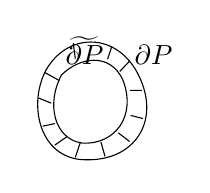
\begin{tikzpicture}[scale=.65]
\draw (0,0) .. controls (-.8,.1) and (-1,1.1) .. (-.65,1.75) .. controls (-.25,2.45) and (.65,2.5) .. (1.1,1.75) .. controls (1.65,.8) and (1.1,-.1) .. (0,0);
\draw (.05,.32) .. controls (-.5,.4) and (-.65,1.1) .. (-.35,1.65) .. controls (0,2) and (.6,2.1) .. (.85,1.55) .. controls (1.12,.85) and (.7,.28) .. (.05,.32);
\draw (-.68,1.7)--(-.39,1.54) (-.8,1.2)--(-.55,1.1) (-.72,.65)--(-.48,.7) (-.48,.28)--(-.25,.44) (-.08,.04)--(.02,.34) (.5,.06)--(.42,.34) (.98,.35)--(.76,.52) (1.24,.8)--(1,.86) (1.22,1.35)--(.99,1.35) (.98,1.92)--(.79,1.72) (.63,2.2)--(.55,1.96) (-.12,2.27)--(-.08,1.97);
\node at (.1,2.12) {$\widetilde{\partial P}$};\node at (1.45,2.05) {$\partial P$};
\end{tikzpicture}}
On a alors \deleted{\unsure{l'isom.} \unsure{à} \unsure{prendre} \unsure{entre}}
\diagram{\begin{tikzcd}[column sep=small]
\deleted{\unsure{\widetilde{\partial P}}}\arrow[r,"{\deleted{\longrightarrow}}" description,draw=none]&\deleted{\unsure{\widetilde{\partial P}}}&\deleted{\partial P'}\arrow[l,"{\deleted{\longleftarrow}}" description,draw=none]&\deleted{P'}\arrow[r,"{\deleted{\longrightarrow}}" description,draw=none]&\deleted{P}
\end{tikzcd}}
\deleted{équivalences d'homotopie}
\mspage{2}
\scanpage{4}
\begin{center}- 45 -\end{center}
\hfill n$^\circ$ 387

7) Soient $K$ un corps, $v$ une valuation discrète sur $K$ tel que $K$ soit \uline{complet} pour $T_v$ ; on désigne par $A$ et $\underline p$ l'anneau et l'idéal de $v$, par $U=A-\underline p$ l'ensemble des éléments inversibles de $A$. Soit $u$ un isomorphisme de $K$ sur un sous-corps de $K$.

a) Montrer que l'on a $u(\underline p)\subset A$ et $u(U)\subset U$. (Pour prouver le premier point observer pour tout $z\in\underline p$, l'équation $x^n=1+z$ admet une solution dans $A$ pour tout $n>0$, en utilisant le lemme de Hensel ; si on avait $v(u(z))<0$, en déduire que l'entier $v(u(z))$ devrait être divisible par tout entier $n>0$. Déduire alors la seconde assertion de la première).

b) Déduire de a) que, ou bien $u(K^*)\subset U$, ou bien $u$ est continu (considérer l'image par $u$ d'une uniformisante de $v$).

c) Donner un exemple de corps algébriquement clos $\Omega$ tel qu'en prenant $K=\Omega((X))$, $K$ soit isomorphe à un sous-corps de $K$ contenu dans $U\cup\{0\}$ (cf. \uline{Alg.}, chap. V, § 5, exerc. 13).

8) a) Soient $K$ un corps, $v$ une valuation de hauteur 1 sur $K$, $A$ son anneau. Soient $H$ une partie compacte de $K$ (pour la topologie $T_v$) $a\ne0$ un point de $K$. Montrer qu'il existe un polynôme $f\in K[X]$ sans terme constant et tel que $f(a)=1$, $f(H)\subset A$. (Prouver qu'on peut prendre pour $f$ un polynôme de la forme
\[
\inserted{\unsure{<}}1-(1-a^{-1}X)(1-c_1^{-1}X)^{n(1)}\ ..\ (1-c_r^{-1}X)^{n(r)}
\]
où les $c_i$ sont des éléments de $H$ tels que $v(c_i)<v(a)$, convenablement choisis, et les $n(i)$ des entiers $>0$ assez grands).

b) Soit $X$ un espace compact totalement discontinu ; on munit l'anneau $C(X;K)$ des applications continues de $X$ dans $K$ de la topologie de la convergence uniforme. Soit $B$ un sous-anneau de $C(X;K)$ contenant les constantes et séparant les points de $X$ ; montrer que $B$ est dense dans $C(X;K)$ (utiliser a) et \uline{Top. gén.}, chap. X, 2$^{\mathrm e}$ éd., § 4, exerc. 21 b)).

9) Soient $A$ un anneau de valuation discrète, $\pi$ une uniformisante de $A$, $K$ le corps des fractions de $A$ ; on suppose $A$ \uline{complet} pour la topologie $\pi$-adique. Les $A$-modules injectifs (\uline{Alg.}, chap. II, 3$^{\mathrm e}$ éd., § 2, exerc. 11) sont identiques aux $A$-modules divisibles (\uline{Alg.}, chap. VII, § 2, exerc. 3) et sont sommes directes
\mspage{3}
\scanpage{5}
\deleted{De plus, l'inclusion $(P,\widetilde{\partial P})\subset(P,\partial P)$ induit un hom de suites exactes}
\diagram{\begin{tikzcd}[column sep=small]
{}\arrow[r]&\deleted{H_!^i(P-\widetilde{\partial P})}\arrow[r]\arrow[d]&\deleted{H^i(P)}\arrow[r]\arrow[d,phantom,"{\deleted{=}}"{rotate=90}]&\deleted{H^i(\widetilde{\partial P})}\arrow[r]\arrow[d,"{\deleted{\simeq}}"]&\deleted{\cdots}\\
{}\arrow[r,dash]&\deleted{H_!^i(P-\partial P)}\arrow[r]&\deleted{H^i(P)}\arrow[r]&\deleted{H^i(\partial P)}\arrow[r]&\deleted{\cdots}
\end{tikzcd}}
\deleted{donc le lemme des cinq donne}
\[
\deleted{H_!^i(P-\widetilde{\partial P})\simeq H^i(P-\partial P)}
\]
\margin{\diagram{\begin{tikzcd}[column sep=small,row sep=small]
&\partial P'\arrow[d,hook]\\
&\widetilde{\partial P}-\partial P\unsure{\simeq}\arrow[dl,hook]\arrow[dr,hook]\\
\widetilde{\partial P}&&\widetilde{\partial P}-\partial P-\partial P'\arrow[dl,hook]\\
&\widetilde{\partial P}-\partial P'\arrow[ul,hook]\arrow[d,phantom,"{\unsure{=P-P'}}"]\\
&\partial P\arrow[u,hook]
\end{tikzcd}}}
\margin{\diagram{\begin{tikzcd}[column sep=small,row sep=small]
&P-P'=\widetilde{\partial P}-\partial P'\arrow[d,hook]\\
\partial P\arrow[ur,hook]\arrow[r,hook]&\widetilde{\partial P}&\partial P'\arrow[l,hook]\arrow[dl,hook]\\
&\widetilde{\partial P}-\partial P\arrow[u,hook]
\end{tikzcd}}
\unsure{équivalences|équivalence} \unsure{d'}}
\diagram{\begin{tikzcd}[column sep=small]
{}\arrow[r]&H^i_{\unsure{P'}}(P,F)\arrow[r]\arrow[d]&H^i(P,F)\arrow[r,dash]\arrow[d,Rightarrow]&H^{\unsure{i}}(P-P',F)\arrow[r]\arrow[d,leftrightarrow,"\simeq"]&\cdots\\
{}\arrow[r]&H^i(P/\partial P;F)\arrow[r]&H^i(P,F)\arrow[r]&\begin{gathered}\deleted{H^i(\unsure{\partial P})}\\H^i(\partial P,F)\end{gathered}\arrow[r]&{}
\end{tikzcd}}
\margin{\diagram{\left\{\begin{tikzcd}[row sep=small]
(P,P-P')\\
(P,\partial P)\arrow[u]
\end{tikzcd}\right.}}
En somme
\[
H^i_{P'}(P,F)\simeq H^i(P\mathbin{\mathrm{mod}}\partial P,F)\simeq H_!^i(\mathring P,F)
\]
En somme on a
\[
H^i_{P'}(P,F)\xrightarrow{\simeq}H^i_{\unsure{?}}(\unsure{P'|\mathring P'},\deleted{\unsure{\mathrm{mod}}}\partial P',F)\simeq H_!^i(\mathring P',F)
\]
grâce à l'inclusion $(P',\partial P')\longrightarrow(P,P-P')$.
\mspage{4}
\scanpage{6}
\begin{center}- 42 -\end{center}
\hfill n$^\circ$ 387
\begin{center}§ 5.\end{center}

1) Soient $A$ un anneau intègre, $K$ son corps des fractions, $T$ une topologie linéaire sur $A$ (chap. III, § 2, exerc. 21).

a) Pour que les voisinages de $0$ pour $T$ constituent un système fondamental de voisinages de $0$ pour une topologie $T_K$ compatible avec la structure d'anneau de $K$, il faut et il suffit que $T$ soit la topologie $T_u(A)$ (chap. III, § 2, exerc. 24) ; $A$ est alors une partie bornée pour $T_K$ et $T_K$ est une topologie séparée localement bornée (\uline{Top. gén.}, chap. III, \unsure{3|2}$^{\mathrm e}$ éd., § 6, exerc. 12 et 20e). Pour que $K$ soit complet (resp. linéairement compact, resp. strictement linéairement compact (chap. III, § 2, exerc. 21)) pour $T_K$, il faut et il suffit que $A$ le soit pour $T$.

b) Pour que la topologie $T_K$ (où $T=T_u(A)$) soit compatible avec la structure de corps de $K$, il faut et il suffit que le radical $\underline R(A)$ de $A$ soit $\ne0$.

\textsuperscript{*}2) Soient $K$ un corps (commutatif), $T$ une topologie séparée sur $K$, compatible avec la structure d'anneau de $K$. Pour que la topologie $T$ soit définie par une valuation de $K$ ou une valeur absolue sur $K$, il faut et il suffit que $T$ soit localement rétrobornée (\uline{Top. gén.}, chap. III, 3$^{\mathrm e}$ éd., § 6, exerc. 22. S'il existe dans $K$ des éléments topologiquement nilpotents utiliser l'exerc. 22 d) de \uline{Top. gén.}, chap. III, 3$^{\mathrm e}$ éd., § 6 et l'exerc. 13 de \uline{Top. gén.}, chap. IX, 2$^{\mathrm e}$ éd., § 3. Dans le cas contraire, utiliser l'exerc. 22 f) de \uline{Top. gén.}, chap. III, 3$^{\mathrm e}$ éd., § 6). *

\textsuperscript{*}3) Soient $A$ un anneau noethérien intègre, $K$ son corps des fractions, $T$ la topologie $T_u(A)$ sur $A$, $T_K$ la topologie correspondante sur $K$ (exerc. 1).

a) Si $A$ est un anneau de Zariski de radical $\underline r\ne0$ et si $A$ est complet pour la topologie $\underline r$-adique, montrer que $A$ est complet pour la topologie $T_u$ (\uline{Top. gén.}, chap. III, 3$^{\mathrm e}$ éd., § 3, n$^\circ$ 5, cor. 2 de la prop. 9).

b) On suppose que $T_K$ est non discrète et est définie par une valuation $v$ de $K$. Montrer alors que $v$ est une valuation discrète et que $A$ est un sous-anneau ouvert de l'anneau $V$ de $v$ ; réciproque. (En utilisant l'hypothèse, qui entraîne $A\ne K$, et la prop. 4 du § 4, n$^\circ$ 1, on peut supposer que $A\subset V$. En utilisant
\mspage{5}
\scanpage{7}
$W$ variété \deleted{\unsure{par}}

$P\subset W$ sous-variété à bord telle que $P=\overline{\mathring P}$.

Soit $Q=P-\mathring P$.

Alors $Q$ est une sous-variété à bord satisfaisant $Q=\overline{\mathring Q}$, et
\[
\unsure{\alpha}\qquad W=P\cup Q,\qquad P\cap Q=\partial P=\partial Q.
\]
Si $W$ est purement de \unsure{dim|codim} $n$, alors $P$ et $Q$ aussi, et $P\cap Q=\partial P=\partial Q$ est purement de \unsure{dim|codim} $n-1$.

Soit $R=\partial P=\partial Q$. On \deleted{\unsure{précisera}} a donc
\[
W-R=\mathring P\amalg\mathring Q.
\]
\[
\deleted{\unsure{H^i(W)}\longrightarrow\unsure{H^i(W,F)}}
\]
La suite exacte de coh. relative pour $W,R,W-R$ donne
\margin{\diagram{\begin{tikzcd}[column sep=small,row sep=small]
&&\mathring Q\arrow[d]\\
&W\arrow[r]\arrow[d]&Q\arrow[d]\\
\mathring P&P\arrow[l]\arrow[r]&P\cap Q=\unsure{R}\arrow[d,phantom,"="{rotate=90}]\\
&&\partial P=T
\end{tikzcd}}}
\diagram{\begin{tikzcd}[column sep=small]
\cdots\arrow[r]&H^i(W,F)\arrow[r]&H^i(W-R,F)\arrow[r]\arrow[d,phantom,"="{rotate=90}]&H^{\unsure{i}}(R,F\otimes\unsure{\mathcal T|\tau}_{T/W})\arrow[r]&H^{i+1}(W,F)\\
&&H^i(\mathring P)\times H^i(\mathring Q)\arrow[d,phantom,"="{rotate=90}]\\
&&H^i(P)\times H^i(Q)
\end{tikzcd}}
\margin{faisceau d'orientation normale à $T$ dans $W$, ici $\simeq\mathbf Z_T$}

Cette suite exacte relative n'est sans doute autre que la suite exacte de Mayer-Vietoris associée à $\unsure{\alpha}$,

On a aussi [\unsure{en faisant} transposée]
\diagram{\begin{tikzcd}[column sep=small]
\cdots\arrow[r]&H_!^i(W-\unsure{T},F)\arrow[r]\arrow[d,phantom,"\simeq"{rotate=90}]&H_!^i(W,F)\arrow[r]&H_!^i(R,F)\arrow[r]&\cdots\\
&H_!^i(\mathring P,F)\times H_!^i(\mathring Q,F)\arrow[d,phantom,"\simeq"{rotate=90}]\\
&H^{n-i}(\mathring P,F^\vee\otimes\unsure{\mathcal T|\tau}_W)^\vee\times H^{n-i}(\mathring Q,F^\vee\otimes\unsure{\mathcal T|\tau}_W)^\vee\arrow[d,phantom,"\simeq"{rotate=90}]\\
&H^{n-i}(P,F\otimes\unsure{\mathcal T|\tau}_W)^\vee\times H^{n-i}(\unsure{Q|R},F^\vee\otimes\unsure{\mathcal T|\tau}_W)^\vee
\end{tikzcd}}
\mspage{6}
\scanpage{8}
\begin{center}- 44 -\end{center}
\hfill n$^\circ$ 387

mais que $K_{\unsure{o|0}}$ n'est pas linéairement compact (cf. § 10, exerc. 2).

6) a) Soient $A$ un anneau de valuation, $M$ un $A$-module, $M'$ un sous-module de $M$. Montrer que pour que $M'$ soit un sous-module \uline{pur} de $M$ (chap. I, § 2, exerc. 24), il faut et il suffit que pour tout $\alpha\in A$, on ait $M'\cap(\alpha M)=\alpha M'$.

b) Soit $M'$ un sous-module pur de $M$, tel que si on munit $M'$ de la topologie dont les $\alpha M'$ (où $\alpha\in A$, $\alpha\ne0$) forment un système fondamental de voisinages de $0$, $M'$ soit linéairement compact. Montrer que pour tout élément $x\in M$, il existe un $y'\in M'$ tel que $x'=x+y'$ ait la propriété suivante : pour tout $\alpha\in A$ tel que $x+M'\in\alpha(M/M')$, on a $x'\in\alpha M$. (Pour chacun des $\alpha\in A$ tels que $x+M'\in\alpha(M/M')$, considérer la partie $S_\alpha$ de $M'$ formée des $y'_\alpha$ tels que $x+y'_\alpha\in\alpha M$).

c) On suppose que $A$ soit un anneau de valuation linéairement compact ; soit $K$ le corps des fractions de $A$. Montrer que si $M$ est un $A$-module sans torsion tel que $M_{(K)}$ admette une base dénombrable, $M$ est somme directe d'une famille dénombrable de $A$-modules de rang 1. (Considérer $M$ comme réunion d'une suite croissante $(M'_i)$ de sous-modules purs tels que $M'_i$ soit de rang $i$, et pour chaque $i$, appliquer b) à $M'_i$ et à son sous-module $M'_{i-1}$).

d) Les hypothèses sur $A$ et $M$ étant les mêmes que dans c), soit $N$ un sous-module pur de $M$, de rang fini. Montrer que $N$ est facteur direct de $M$ (observer que tout $A$-module qui est somme directe d'un nombre fini de $A$-modules de rang 1 est linéairement compact et utiliser b)).

e) Les hypothèses sur $M$ et $M'$ étant celles de b), montrer que pour tout $x\in M$, il existe $y'\in M'$ tel que l'annulateur de $x'=x+y'$ soit égal à l'annulateur de l'élément $x+M'\in M/M'$. (Soit $\underline a$ l'annulateur de $x+M'$ ; pour tout $\alpha\in\underline a$, soit $T_\alpha$ la partie de $M'$ formée des $y'$ tels que $\alpha(x+y')=0$, et montrer que l'intersection des $T_\alpha$ n'est pas vide).

f) On suppose que $A$ soit un anneau de valuation tel que pour tout idéal $\underline a\ne0$, le $A$-module $A/\underline a$ soit linéairement compact (pour la topologie discrète). Montrer que tout $A$-module de torsion de type fini $M$ est somme \unsure{directe.d'un|directe d'un} nombre fini de $A$-modules monogènes. (Si $(z_i)_{1\le i\le n}$ est un système de générateurs de $M$, raisonner par récurrence sur $n$, en considérant un des $z_i$ dont l'annulateur est le plus petit et en remarquant que le sous-module de $M$ qu'il engendre est pur).
\mspage{7}
\scanpage{9}
Ecrivons aussi les 2 suites exactes relatives à l'inclusion $P\subset W$. On a
\diagram{\begin{tikzcd}[column sep=small]
\cdots\arrow[r]&H^i_P(W,F)\arrow[r]\arrow[d,"{\deleted{\simeq}}"]&H^i(W,F)\arrow[r,dash]&H^i(W-P,F)\arrow[r,dash]\arrow[d,phantom,"="{rotate=90}]&\cdots\\
&\deleted{H^i_{\unsure{!}}(\mathring P)}&&H^i(\mathring Q,F)\\
&&&H^i(Q,F)\arrow[u,"\simeq"]
\end{tikzcd}}
\margin{\deleted{\unsure{si} \unsure{compact}}}

Or, si $\widetilde P$ est un petit épaississement de $P$ dans $W$, alors l'inclusion $P\longrightarrow\widetilde P$ induit, on le sait
\figure{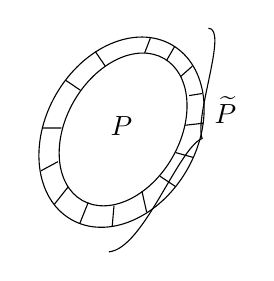
\begin{tikzpicture}[scale=.8]
\begin{scope}[rotate=-30]
\draw (0,0) ellipse (1.2 and 1.6);\draw (0,.05) ellipse (.9 and 1.3);
\draw (-.35,1.52)--(-.31,1.27) (.05,1.6)--(.05,1.35) (.45,1.47)--(.37,1.23) (.8,1.17)--(.64,1.04) (1.05,.77)--(.82,.6) (1.18,.22)--(.91,.15) (1.18,-.32)--(.88,-.3) (.98,-.9)--(.75,-.65) (.62,-1.37)--(.48,-1.07) (.15,-1.58)--(.1,-1.23) (-.35,-1.52)--(-.3,-1.18) (-.8,-1.17)--(-.64,-.91) (-1.12,-.57)--(-.86,-.42) (-1.18,.27)--(-.9,.25) (-1,.9)--(-.75,.78);
\end{scope}
\node at (0,.1) {$P$};
\draw (1.38,1.65) .. controls (1.7,1.65) and (1.15,.25) .. (1.28,-.1) .. controls (.9,-.25) and (.35,-1.85) .. (-.2,-1.9);
\node at (1.65,.35) {$\widetilde P$};
\end{tikzpicture}}
\diagram{\begin{tikzcd}[column sep=large]
H^i_P(\widetilde P,F)\arrow[r,"\simeq"]\arrow[d,phantom,"\simeq"{rotate=90},"\text{excision}"']&H^i(\widetilde P\mathbin{\mathrm{mod}}\partial\widetilde P,F)\arrow[d,phantom,"\simeq"{rotate=90}]\\
H^i_P(W,F)&H_!^i(\mathring P,F)
\end{tikzcd}}
Donc la suite exacte pour l'inclusion $P\subset W$ peut s'écrire
\diagram{\begin{tikzcd}[column sep=small]
\cdots\arrow[r,dash]&H_!^i(\mathring P,F)\arrow[r,dash]\arrow[d,phantom,"\simeq"{rotate=90}]&H^i(W,F)\arrow[r,dash]&H^i(Q,F)\arrow[r,dash]&\cdots\\
&H^{n-i}(P,F^\vee\otimes\unsure{\mathcal T|\tau}_W)^\vee
\end{tikzcd}}
\mspage{8}
\scanpage{10}
\begin{center}- 43 -\end{center}
\hfill n$^\circ$ 387

le fait que $A$ est ouvert pour $T_K$, montrer que $V$ est un $A$-module de type fini et conclure à l'aide du § 3, n$^\circ$ 5, prop. 9. Pour la réciproque, on observera que $A$ est un anneau local dont l'idéal maximal $\underline m$ et $(0)$ sont les seuls idéaux premiers, et dans lequel tout idéal $\underline a\ne0$ est par suite $\underline m$-primaire). La clôture intégrale de $A$ est alors $V$. Donner un exemple où $A\ne V$ (prendre pour $V$ un anneau de $A$ est alors $V$. Donner un exemple où $A\ne V$ (prendre pour $V$ un anneau de séries formelles $k[[T]]$, où $k$ est un corps).

c) En déduire un exemple de corps topologique complet non discret, dont la topologie n'est pas localement rétrobornée (utiliser b) et l'exerc. 2).

4) Soient $v$ une valuation sur un corps $K$, $A$ son anneau, $\underline m$ son idéal maximal.

a) Pour que la topologie définie par $v$ sur $A$ soit identique à la topologie $\underline m$-adique, il faut et il suffit que $A$ soit un corps ou un anneau de valuation discrète.

b) Pour que la topologie définie par $v$ fasse de $A$ un anneau strictement linéairement compact (chap. III, § 2, exerc. 21), il faut et il suffit que $A$ soit un corps ou un anneau de valuation discrète (utiliser a) et le chap. III, § 2, exerc. 22 a)).

\textsuperscript{*}5) a) Soient $K$ un corps, $v$ une valuation sur $K$, $\Gamma$ le groupe des ordres de $v$. Pour que $K$ soit linéairement compact (chap. III, § 2, exerc. 15) pour la topologie $T_v$, il faut et il suffit que pour toute partie \uline{bien ordonnée} $B$ de $\Gamma$ et toute famille $(a_\beta)_{\beta\in B}$ d'éléments de $K$ telle que, pour $\lambda<\mu<\nu$, on ait $v(a_\lambda-a_\mu)<v(a_\mu-a_\nu)$, il existe un élément $a\in K$ tel que $v(a-a_\lambda)=v(a_\lambda-a_\mu)$ pour tout couple d'indices $\lambda,\mu$ tels que $\lambda<\mu$. (Utiliser l'exerc. de \uline{Ens.}, chap. III, 2$^{\mathrm e}$ éd., § 2). Lorsqu'il en est ainsi, l'anneau $A$ de la valuation $v$ est aussi linéairement compact pour la topologie discrète.

b) Montrer que le corps valué $S(\Gamma,k)=K$ défini au § 3, exerc. 2, est linéairement compact pour $T_v$. On prend pour $\Gamma$ le groupe totalement ordonné $\underline Q$ des nombres rationnels, et on considère le sous-anneau $K_{\unsure{o|0}}$ de $K$ formé des $x=(x_\alpha)$ tels que l'ensemble des $\alpha\in\underline Q$ pour lesquels $x_\alpha\ne0$ soit fini ou soit l'ensemble des points d'une suite strictement croissante tendant vers $+\infty$. Montrer que $K_{\unsure{o|0}}$ est un corps qui est complet pour la valuation $v_{\unsure{o|0}}$ induite par la valuation canonique $v$ de $K$, et que $v_{\unsure{o|0}}$ a même groupe des valeurs et même corps résiduel que $v$,
\mspage{9}
\scanpage{11}
\diagram{\begin{tikzcd}[column sep=small,row sep=large]
&H^{i-1}(R,F\arrow[dl]\arrow[dr]\arrow[dd]&\\
H^{n-i}(P,F^\vee\otimes\unsure{\mathcal T|\tau}_W)^\vee\simeq H_!^i(\mathring P,F)\arrow[dr]&&H_!^i(\mathring Q,F)\simeq H^{n-i}(Q,F^\vee\otimes\unsure{\mathcal T|\tau}_W)^\vee\arrow[dl,very thick]\\
&H^i(W,F)\arrow[dl,very thick]\arrow[dr,very thick]&\\
H^i(P,F)\arrow[dr]&&H^i(Q,F)\arrow[dl]\\
&H^i(R,F)&
\end{tikzcd}}
\margin{\diagram{\boxed{\begin{tikzcd}[row sep=large,column sep=large]
{}\arrow[dr,leftrightarrow,"\begin{gathered}\text{suite exacte}\\\text{de coh. à supports}\\\deleted{\unsure{ordinaires}}\ \text{pour }P\subset W\end{gathered}","\begin{gathered}\text{suite exacte}\\\text{de cohomologie ! pour}\\Q\subset W\end{gathered}"']&\\
&{}
\end{tikzcd}}}}
\diagram{\boxed{\begin{tikzcd}[column sep=large,row sep=small]
S_!(W,R)&\text{duale de}&S(W,R)\arrow[d]\\
S(W,\unsure{P})\arrow[u]\arrow[d,phantom,"\simeq"{rotate=90}]&\text{duale de}&S(W,Q)\arrow[d,phantom,"\simeq"{rotate=90}]\\
S_!(W,Q)&\text{duale de}&S_!(W,P)\arrow[d]\\
S(W,R)\arrow[u]\arrow[d,phantom,"\simeq"{rotate=90}]&\text{duale de}&S_!(W,R)\arrow[d,phantom,"="{rotate=90}]\\
MV(W;P,Q)&&MV_!(W,R)
\end{tikzcd}}}
\margin{\deleted{1° Suite exacte de Mayer Vietoris $P,Q,P\cap Q=\unsure{S\times T|R=T},W$}

\deleted{2° Suite exacte de coh. relative}
\diagram{\begin{tikzcd}[row sep=small]
\deleted{H_Q^i(W)}\arrow[r,"{\deleted{\longrightarrow}}" description,draw=none]\arrow[d,phantom,"{\deleted{\simeq\ ?}}"{rotate=90}]&\deleted{H^i(W)}\arrow[r,"{\deleted{\longrightarrow}}" description,draw=none]&\deleted{H^i(W-Q)}\arrow[d,phantom,"{\deleted{\simeq}}"{rotate=90}]\\
\deleted{H_!^i(W-P)}\arrow[d,phantom,"{\deleted{=}}"{rotate=90}]&&\deleted{H^i(P)}\\
\deleted{H_!^i(Q-\partial Q)}\arrow[d,phantom,"{\deleted{\simeq}}"{rotate=90}]\\
\deleted{(H^{\unsure{n-i}}(Q\unsure{-|,}\partial Q))^\vee}\arrow[d,phantom,"{\deleted{=}}"{rotate=90}]\\
\deleted{H^{n-i}(Q)^\vee}
\end{tikzcd}}
\[\deleted{H_Q^i(W)\times H^{\unsure{n-i}}(Q\unsure{+|,}}\]}

\uline{Récapitulation}
\diagram{\boxed{\begin{tikzcd}[column sep=small]
&\Psi\arrow[dl]\arrow[dr]&\\
\Phi\arrow[dr]&&\Phi'\arrow[dl]\\
&\Psi'&
\end{tikzcd}}}
\diagram{\boxed{\begin{array}{rll}
\Psi:&H(P),H(Q),H(T),H(W)\\
\Psi':&\unsure{H}\mathbin{-}\text{duals}\mathbin{-}\\
\Phi:&H(P)^\vee,H(Q),H(W)&\deleted{(\text{pas de }H(T))}\\
\Phi':&H(P),H(Q)^\vee,H(W)&(\text{pas de }H(T))
\end{array}}}
\[
\left.\begin{aligned}
\Phi&\simeq S(W,P)\simeq S_!(W,Q)\\
\Phi'&\simeq S(W,Q)\simeq S_!(W,P)
\end{aligned}\right\}\ (\Phi,\Phi'\text{ duals})
\]
\[
\left.\begin{aligned}
\Psi&\simeq S(W,T)\simeq MV(W;P,Q)\\
\Psi'&\simeq S_!(W,T)\simeq MV_!(W,P,Q)
\end{aligned}\right\}\ (\Psi,\Psi'\text{ duals})
\]
\mspage{10}
\scanpage{12}
\margin{\unsure{W|11}}
\begin{center}- 46 -\end{center}
\hfill n$^\circ$ 387

de $A$-modules isomorphes, soit à $K$, soit à $K/A$ (\uline{Alg.}, chap. VII, § 2, exerc. 3). En outre, tout $A$-module monogène est isomorphe à un sous-module de $K/A$. On appelle \uline{dual torique} (\uline{algébrique}) d'un $A$-module $M$ le $A$-module $\operatorname{Hom}_A(M,K/A)$, que l'on note $M^*$ ; l'application canonique $c_M:M\longrightarrow M^{**}$ est injective (\uline{Alg.}, chap. II, 3$^{\mathrm e}$ éd., § 2, exerc. 13 b)). Pour tout sous-module $N$ de $M$, le sous-module $N^\circ$ de $M^*$ formé des $u$ tels que $u(x)=0$, est appelé l'\uline{orthogonal} de $N$ dans $M^*$ ; le dual de $M/N$ s'identifie canoniquement à $N^\circ$ et le dual de $N$ à $M^*/N^\circ$. Le dual torique d'une limite inductive $\varinjlim M_\alpha$ est canoniquement isomorphe à la limite projective $\varprojlim M_\alpha^*$.

a) On sait que les $A$-modules de rang un (\uline{Alg.}, chap. VII, § 4, exerc. 22) sont isomorphes à un module de l'une des formes $A$, $K$, $K/A$ ou $A/\pi^h A$. Montrer que les duals toriques algébriques de $K$ ou de $A/\pi^h A$ leur sont respectivement isomorphes, que le dual torique de $A$ est isomorphe à $K/A$ et que celui de $K/A$ est isomorphe à $A$ (on utilisera la connaissance des sous-$A$-modules de $K$ et le fait que $A$ est complet (pour le dual de $K/A$)). En déduire que pour tout $A$-module $M$ de rang fini, $M^*$ est un module de même rang et que l'homomorphisme canonique $c_M$ est bijectif.

b) Soient $M$ un $A$-module, $N$ un sous-module de rang fini de $M$. Montrer que l'orthogonal de $N^\circ$ dans $M^{**}$ s'identifie (par $c_M$) à $N$ (utiliser a)).

c) Montrer qu'un $A$-module qui est noethérien (resp. artinien) est de rang fini (plonger $M$ dans son enveloppe injective (\uline{Alg.}, chap. II, 3$^{\mathrm e}$ éd., § 2, exerc. 18)) $M^*$ est alors artinien (resp. noethérien).

d) On désigne par $\sigma(M^*,M)$ la topologie (sur $M^*$) de la convergence simple dans $M$ ($K/A$ étant muni de la topologie discrète). Montrer que si $N$ est un sous-module de $M$, $\sigma(N^\circ,M/N)$ est induite sur $N^\circ$ par $\sigma(M^*,M)$, et que $\sigma(M^*/N^\circ,N)$ est quotient par $N^\circ$ de la topologie $\sigma(M^*,M)$. (Pour le second point, on notera que si $P$ est un sous-module de $M$ tel que $N\subset P\subset M$, le dual de $P/N$ s'identifie à $N^\circ/P^\circ$). Si $M=\varinjlim M_\alpha$ la top ologie $\sigma(M^*,M)$ est limite projective des topologies $\sigma(M_\alpha^*,M_\alpha)$.

e) Les topologies $\sigma(K,K)$ et $\sigma(A,K/A)$ sont les topologies $\pi$-adiques ; les topologies $\sigma(A/\pi^h A,A/\pi^h A)$ et $\sigma(K/A,A)$ sont les topologies discrètes. En déduire que pour tout $A$-module $M$, le module $M^*$, muni de $\sigma(M^*,M)$ est \uline{linéairement compact} (chap. III, § 2, exerc. 15 ; on considérera $M$ comme module quotient d'un $A$-module libre).
\scanpage{13}
Soit $W$ une variété \deleted{topologique} diff.

$P,Q$ deux sous-variétés à bord

avec
\[
P\cap Q=\partial P=\partial Q
\]
\[
P\cup Q=W
\]
et $P$ et $Q$ étant \unsure{deux|des} fibrés diff.

\deleted{Alors on a}
\margin{$\partial P$}
\margin{\deleted{\unsure{W}}}
\diagram{\begin{tikzcd}[column sep=small]
P\arrow[r]&S&Q\arrow[r]&T\\
M\arrow[u,hook]&&N\arrow[u,hook]
\end{tikzcd}}
de bases $S,T$ des variétés diff \unsure{cptes} $S,T$, de fibres des variétés à bords $M$, resp. $N$. Donc $\partial P$ est un fibré sur $S$ de fibre $\partial M$, et $\partial Q$ un fibré sur $T$ de fibre $\partial N$ :
\diagram{\begin{tikzcd}[column sep=small]
\partial P\arrow[r]&S&\partial Q\arrow[r]&T\\
\partial M\arrow[u,hook]&&\partial N\arrow[u,hook]
\end{tikzcd}}
On suppose donnés des isomorphismes
\[
\alpha:S\simeq\partial N\qquad\beta:T\simeq\partial M
\]
et \deleted{pour les fibres} des trivialisations
\[
\sigma:\partial P\simeq S\times\partial M\qquad\tau:\partial Q\simeq T\times\partial N
\]
D'où, par composition
\[
(\alpha,\sigma):\partial P\simeq\partial N\times\partial M,\quad(\beta,\tau):\partial Q\simeq\partial M\times\partial N
\]
et par suite un isom
\[
\varphi:\partial P\simeq\partial Q
\]
\mspage{12}
\scanpage{14}
\begin{center}- 48 -\end{center}
\hfill n$^\circ$ 387

f) Soit $M$ un $A$-module topologique linéairement compact ; montrer que l'injection canonique $M\longrightarrow(M')^*$ est une \uline{bijection}, et que la topologie de $M$ (identifié à $(M')^*$) est égale à $\sigma(M,M')$. (Observer que si $U$ est un sous-module ouvert de $M$, $M/U$ est artinien par a), et par suite $U^\circ$ est noethérien (exerc. 9 c)), et en déduire l'identité des topologies considérées sur $M$ ; terminer à l'aide de e)).

g) Soient $M$, $N$ deux $A$-modules topologiques dont les topologies sont linéaires ; pour tout homomorphisme \uline{continu} $u:M\longrightarrow N$, on a ${}^tu(N')\subset M'$, et on désigne encore par ${}^tu$ (par abus de notation) l'application linéaire de $N'$ dans $M'$ ayant même graphe que ${}^tu$. Si $M$ et $N$ sont séparés, montrer que la restriction à $M$ de ${}^t({}^tu)$ coïncide avec $u$ ($M$ et $N$ étant respectivement considérés comme plongés canoniquement dans $(M')^*$ et $(N')^*$) ; en outre, pour tout sous-module fermé $Q$ de $N$, on a $(u^{-1}(Q))^\circ\cap M'={}^tu(Q^\circ)$ (utiliser e)).

h) Soit $M$ un $A$-module linéairement compact ; déduire de g) et de l'exerc. 9 f) que, pour que $M$ soit sans torsion, il faut et il suffit que $M'$ soit divisible, et pour que $M$ soit divisible, il faut et il suffit que $M'$ soit sans torsion.

\begin{center}\unsure{-:-:-:-}\end{center}
\mspage{13}
\scanpage{15}
Ceci posé, on \unsure{suppose} $W$ construit en recollant $P$ et $Q$ suivant leurs bords \deleted{\unsure{communs}} via $\varphi$.

\deleted{\unsure{On peut}}

\deleted{\unsure{On aura}}

L'hypothèse que $\partial P$ est un fibré trivial sur $S$ implique que l'inclusion \deleted{\unsure{un}}
\diagram{\begin{tikzcd}
W-Q=P-\partial P \arrow[r,hook] & P
\end{tikzcd}}
est un isomorphisme d'homotopie,

\deleted{\unsure{En fait}}

et de même pour
\diagram{\begin{tikzcd}
W-P=Q-\partial Q \arrow[r,hook] & Q & \text{''\qquad ''\qquad ''}.
\end{tikzcd}}

\deleted{\unsure{On a donc}}

Considérons le diagramme
\diagram{\begin{tikzcd}[row sep=large,column sep=large]
& & T=\partial M & t \arrow[l,very thick] \\
& W & Q \arrow[l,hook] \arrow[u,"\unsure{\simeq|2}"] & N=D_{\unsure{1}}\sim e \arrow[l,hook] \arrow[u,hook,very thick] \\
\partial N=S^1 & P \arrow[l] \arrow[u,hook,very thick] & {\begin{gathered}S^1\times T=\partial N\times\partial M\deleted{\unsure{\partial}}\\=\partial P=\partial Q=P\cap Q\end{gathered}} \arrow[l,hook] \arrow[u,hook] & \partial N=\unsure{S^1} \arrow[l,hook] \arrow[u,hook] \\
s \arrow[u] & M \arrow[l] \arrow[u,hook] & \partial M=T \arrow[l,hook] \arrow[u,hook] & (s,t) \arrow[l,hook] \arrow[u,hook]
\end{tikzcd}}
\mspage{14}
\scanpage{16}
\begin{center}- 47 -\end{center}
\hfill n$^\circ$ 387

f) Soient $M$, $N$ deux $A$-modules ; pour tout homomorphisme $u:M\longrightarrow N$, on note ${}^tu$ l'homomorphisme $\operatorname{Hom}(u,1_{K/A})$ de $N^*$ dans $M^*$, tel que $({}^tu(w))(x)=w(u(x))$ pour tout $x\in M$ et tout $w\in N^*$ ; ${}^tu$ est continu pour les topologies $\sigma(N^*,N)$ et $\sigma(M^*,M)$. Si $u$ est l'endomorphisme $x\longrightarrow\pi x$ de $M$, ${}^tu$ est l'endomorphisme $w\longrightarrow\pi w$ de $M^*$. Pour tout sous-module $P$ de $M$, on a $(u(P))^\circ={}^tu^{-1}(P^\circ)$.

10) Les hypothèses et notations sont celles de l'exerc. 9.

a) Si $M$ est un $A$-module \uline{topologique} discret, montrer que $M$ est un module de torsion. Si de plus $M$ est linéairement compact, montrer que $M$ est artinien (si $N$ est le noyau de l'endomorphisme $x\longrightarrow\pi x$, observer que $N$ est linéairement compact et discret, et peut être considéré comme $(A/\pi A)$-espace vectoriel ; utiliser alors l'exerc. 20 d) du chap. II, \S 2).

b) Déduire de a) que tout $A$-module topologique linéairement compact est strictement linéairement compact (chap. II, \S 2, exerc. 19).

c) On appelle \uline{dual torique topologique} d'un $A$-module topologique $M$ le sous-module $M'$ du dual torique algébrique $M^*$, formé des homomorphismes continus de $M$ dans $K/A$ (ce dernier étant muni de la topologie discrète). Si la topologie de $M$ est linéaire (chap. II, \S 2, exerc. 14) et si $N$ est un sous-module fermé de $M$, montrer que le dual torique topologique de $M/N$ s'identifie à $N^\circ\cap M'$ et celui de $N$ à $M'/(N^\circ\cap M')$ (pour déterminer le dual de $N$, remarquer que pour tout homomorphisme continu $u$ de $N$ dans $K/A$, il existe un sous-module ouvert $U$ de $M$ tel que $u(x)=0$ dans $N\cap U$, puis utiliser l'exerc. 9).

d) Pour un $A$-module topologique $M$ de rang fini, le dual torique topologique $M'$ est égal au dual torique algébrique $M^*$ (se ramener au cas des modules de rang un).

e) Soit $M$ un $A$-module topologique séparé dont la topologie est linéaire ; montrer que pour tout $x\ne0$ dans $M$, il existe un $u\in M'$ tel que $u(x)\ne0$ (remarquer qu'il existe un sous-module ouvert $U$ de $M$ tel que $x\in U$) ; autrement dit, l'application canonique $M\longrightarrow(M')^*$ est injective. En déduire que si $N$ est un sous-module fermé de $M$, $N^\circ\cap M'$ est dense dans $N^\circ$ pour la topologie $\sigma(M^*,M)$ (utiliser d)), et par suite on a $N=M\cap(N^\circ\cap M')^\circ$ dans $M^{**}$. Montrer que $M$ est dense dans $(M')^*$ pour la topologie $\sigma((M')^*,M')$.
\mspage{15}
\scanpage{17}
\diagram{\begin{array}{cccc}
W&P&Q&R\\
V'&\overbrace{X'_{\unsure{\eta|\gamma}}=V'_{\unsure{\eta|\gamma}}}&\unsure{V'_s}&V'_s\times\unsure{\eta|\gamma}
\end{array}}
\diagram{\begin{tikzcd}
& W \arrow[dl,dash] \arrow[dr,dash] & \\
P \arrow[dr,dash] && Q \arrow[dl,dash]\\
& R &
\end{tikzcd}}
\figure{\begin{tikzpicture}\draw (0,0)--(6,0)--(6,-.6)--(12,-.6);\end{tikzpicture}}
\diagram{\begin{array}{cccc}
M&N&T=\dot M,&S=\dot N\\
X'_{\overline{\unsure{\eta|\gamma}}}&\deleted{\unsure{D}}\unsure{\sim}e&V'_s&\unsure{\eta|\gamma}\sim S^1
\end{array}}

\diagram{\begin{tikzcd}[row sep=1.1em,column sep=1.1em,
execute at end picture={
\draw[gray,rotate around={-35:(-1,0)}] (-1,0) ellipse (1.3 and 2.1);
\draw[gray,rotate around={-35:(1.2,0)}] (1.2,0) ellipse (1.3 and 2.1);
\draw[gray,rotate around={-35:(-3,-1.4)}] (-3,-1.4) ellipse (1.1 and 1.7);
\draw[gray,rotate around={-35:(3,-1.4)}] (3,-1.4) ellipse (1.1 and 1.7);
\foreach \x in {0,.25,.5,.75,1,1.25}{\draw (-4.5+\x,-1.2-\x) -- (-5+\x,-2.3-\x);\draw (3+\x,-1.8-\x/2)--(2.4+\x,-2.9-\x/2);}
}]
&&S&&W&&&&\\
s \arrow[urr] &&&P \arrow[ul] \arrow[ur,hook] &&&&T&\\
&M \arrow[ul,very thick] \arrow[urr,hook] &&&&Q \arrow[uul,hook] \arrow[urr] &&&t \arrow[ul]\\
&&T \arrow[ul,hook,very thick] \arrow[rr,hook] &&{\begin{gathered}R\\\Vert\\T\times S\end{gathered}} \arrow[uul,hook,very thick] \arrow[ur,hook] &&&N \arrow[ull,hook] \arrow[ur]&\\
\unsure{s}&&\unsure{s}&&(s,t) \arrow[ull,hook] \arrow[rr,hook] &&S \arrow[ull,hook] \arrow[ur,hook,"\unsure{\times}"'] &&\unsure{T}\\
&&&&\varnothing \arrow[u,hook] &&&t \arrow[ul,very thick] \arrow[ur,dashed,hook]&
\end{tikzcd}}

\margin{$\displaystyle\binom{5}{2}=\frac{5.4.3}{12.}=10$}

\diagram{\begin{tikzcd}
D^1\times B\sim B\\
S^1\times B \arrow[u,hook]
\end{tikzcd}}
\deleted{\diagram{\begin{tikzcd}
& H^{\unsure{n+i}}\\
H^i(B)\times H^{i-1}(B) \arrow[r] \arrow[d] & {}\\
H^i(B &
\end{tikzcd}}}

\margin{\diagram{\begin{array}{ccccc}1&2&3&4&5\\\cdot&\cdot&\cdot&\cdot&\cdot\end{array}}}
\margin{\diagram{\begin{array}{ccc}
123&234&345\\124&235&\\125&245&\\134&\cdot&\\135&&\\145&&
\end{array}}}

\diagram{\begin{tikzcd}[row sep=1.1em,column sep=1.3em,
execute at end picture={
\draw[very thick] (-2.7,1.3)--(-1.4,2.4)--(2.2,-.3)--(.7,-1.7)--cycle;
\draw (-2.55,1.4)--(-1.25,2.5)--(2.35,-.2)--(.85,-1.6);
\draw[gray] (-4,-.4)--(-2.8,.7)--(-.8,-1.4)--(-2,-2.5)--cycle;
\draw (2.2,-1.1)--(3.2,-.1)--(4.1,-.7)--(3.1,-1.8)--cycle;
\foreach \x in {0,.18,.36,.54,.72}{\draw (2.3+\x,-1.15+\x)--(3.1+\x,-1.7+\x);}
}]
&\unsure{\eta|S}&&V'&&V'_s&\\
s \arrow[ur] &&X'_{\unsure{\eta|\gamma}} \arrow[ul] \arrow[ur,hook,very thick] &&V'_s \arrow[ul,hook,very thick] \arrow[ur,"\sim"] &&t \arrow[ul]\\
&X'_{\overline{\unsure{\eta|\gamma}}} \arrow[ul,very thick] \arrow[ur,hook,very thick] &&V'_s\times\unsure{\eta|\gamma} \arrow[ul,very thick] \arrow[ur,very thick] &\unsure{S^1}&&e \arrow[ull,very thick] \arrow[u,"\sim"']\\
&&V'_s \arrow[ul,very thick] \arrow[ur,very thick] &&\unsure{\eta|\gamma} \arrow[ul,very thick] \arrow[urr] &&\unsure{X'_s}\\
\unsure{\cdot}&&&(s,t) \arrow[ul,very thick] \arrow[ur] &&t&
\end{tikzcd}}

\margin{$10+10+2$}
\margin{\diagram{\begin{array}{ccc}
\varnothing&T\sim S&R\\
5+5&2+2&2\\
3&3+3&\\
2+2&1+1&\\
1+2&1+1&\\\hline
\boxed{20}&\boxed{14}&\boxed{2}
\end{array}}}
\margin{\diagram{\begin{array}{c}M\sim N\\2+2\\\hline\boxed4\end{array}}}

\diagram{\begin{tikzcd}[row sep=large,column sep=large]
&H^{i-1}(R) \arrow[dd,very thick]&\\
H^{n-i}(P)^\vee \arrow[dr]& & H^{n-i}(Q)^\vee \arrow[dl]\\
&H^i(W) \arrow[dl,very thick] \arrow[dr]&\\
H^i(P) \arrow[dr]&&H^i(Q) \arrow[dl] \arrow[dr,very thick]&\\
&H^i(R) \arrow[d,dash]&&H^{n-i\unsure{-1}}(P)^\vee\\
&H^{i+1}(W)&&
\end{tikzcd}}
\diagram{\begin{tikzcd}
H^i(Q)\times H^{n-i\unsure{-1}}(P) \arrow[r] & H^{n-1}(R)\simeq\Lambda\\
H^{\unsure{n-i}}(P)^\vee \arrow[r] & H^i(P)
\end{tikzcd}}

\margin{\figure{\begin{tikzpicture}\node[draw,ellipse] {$40$};\end{tikzpicture}} suites exactes de coh. \unsure{relative}}
\margin{et autant pour l'homologie ...}
\margin{Cela fait $80$ suites exactes, mais}
\mspage{16}
\scanpage{18}
FACULTE DES SCIENCES

Institut Henri Poincaré

Département de Mathématiques

11, rue Pierre et Marie Curie

75 - \uline{PARIS 5ème}

\begin{center}
Le Professeur \uline{N. EFIMOV}

Doyen de la Faculté de Mathématiques de MOSCOU
\end{center}

actuellement à PARIS, comme Professeur d'échange, donnera, pendant son séjour,

une série de conférences sur le sujet suivant :

\begin{center}``LE PROBLEME DES IMMERSIONS HYPERBOLIQUES'' .\end{center}

\uline{Première conférence} : jeudi 25 Avril 1968

à 14 heures, salle 116

à l'Institut Henri Poincaré - 11, rue Pierre et Marie Curie - PARIS 5ème.
\mspage{17}
\scanpage{20}
\textcircled{a}
\diagram{\begin{tikzcd}[row sep=large,column sep=large]
& L^{\bullet\,\mathrm{triv}}=\mathbb R\deleted{\unsure{(\Gamma,\pi)}}\Gamma_{\unsure{*}}(W_0)^{\mathrm{triv}} \arrow[dl,dashed] \arrow[r,bend left] & \text{on met dessus op. triviale de $\pi$}\\
{\begin{tikzpicture}[baseline=(current bounding box.center)]\node[draw,ellipse,inner sep=6pt] {$\begin{gathered}[R^\bullet]\\\Vert\\\mathbb R(\Gamma,\pi)_!(\mathring M)\end{gathered}$};\end{tikzpicture}} \arrow[r,dashed] & K^\bullet=\mathbb R(\Gamma,\pi)_{\unsure{*}}(M) \arrow[u,"\rho\ \text{compatible aux cup}"] &
\end{tikzcd}}
\margin{dans catégorie dérivée de $\Lambda[\pi]$}

\textcircled{b} Appliquons $\mathbb R\Gamma^\pi$ à \textcircled{a}, on trouve
\diagram{\begin{tikzcd}[row sep=large,column sep=large]
& {\begin{gathered}L^{\bullet\pi}=\mathbb R\Gamma(W_0\times S^1)\simeq\mathbb R\Gamma(W_0)\overset{\mathrm L}{\otimes}_{\Lambda}\mathbb R\Gamma(S^1)\\\simeq\mathbb R\Gamma(W_0)\times\mathbb R\Gamma(W_0)(-1]\end{gathered}} \arrow[dl,dashed]\\
{\begin{tikzpicture}[baseline=(current bounding box.center)]\node[draw,ellipse,inner sep=6pt] {$\begin{gathered}[R^{\bullet\pi}]\\\Vert\\\mathbb R\Gamma_!(\mathring P)\end{gathered}$};\end{tikzpicture}} \arrow[r,dash,dashed] \arrow[d,equal] & K^{\bullet\pi}=\mathbb R\Gamma(P)=\mathbb R\Gamma(W-W_0) \arrow[u,"(\alpha,\beta)",very thick]\\
\mathbb R\Gamma_!(W-W_0)&
\end{tikzcd}}
\margin{Suite exacte de cohomologie relative pour $(P,\partial P=S^1\times W_0)$}
\diagram{\begin{tikzcd}[column sep=large]
\mathbb R\Gamma(P)\simeq\mathbb R\Gamma(W-W_0) \arrow[r,"\text{compatible aux cup}","\alpha"'] &\mathbb R\Gamma(W_0)\\
\mathbb R\Gamma(P)=\mathbb R\Gamma(W-W_0) \arrow[r,"\beta",very thick] &\mathbb R\Gamma(W_0)(-1)
\end{tikzcd}}
\margin{s'identifie sur la cohomologie au $\partial$ de la suite exacte de \unsure{dévolution} qui relie $H^i(W-W_0)$ et $H^{i-1}(W_0)$ ...}

\textcircled{c} Appliquons foncteur oubli $\omega$ à \textcircled{a}, on trouve
\diagram{\begin{tikzcd}[row sep=large,column sep=large]
&L^\bullet=\mathbb R\Gamma(W_0) \arrow[dl,dashed]\\
{\begin{tikzpicture}[baseline=(current bounding box.center)]\node[draw,ellipse,inner sep=6pt] {$\begin{gathered}[R^\omega]\\\Vert\\\mathbb R\Gamma_!(\mathring M)\end{gathered}$};\end{tikzpicture}} \arrow[r,dash,dashed] & K^{\bullet\omega}=\mathbb R\Gamma(M) \arrow[u,"\text{compatible aux cup}"]
\end{tikzcd}}

\textcircled{d}
\margin{NB. c'est le $\beta$ de \textcircled{b}}
\diagram{\begin{tikzcd}[row sep=large,column sep=large]
&\mathbb R\Gamma(P)\simeq\mathbb R\Gamma(W-W_0) \arrow[dl,"\beta"',very thick]\\
\mathbb R\Gamma(W_0)(-2] \arrow[r] & [\mathbb R\Gamma_!(W)] \arrow[u,"\rho\ \text{compatible avec cup}"']
\end{tikzcd}}
[Suite exacte en \unsure{Cohomologie|cohomologie} relative pour $(W,W-W_0)$, ou au choix pour $(W,P)$]
\margin{Permet de trouver $\mathbb R\Gamma(W)$ en fonction de \textcircled{a}}
\mspage{19}
\scanpage{21}
\begin{center}-4.15-\end{center}

$V_5$ into $V_5$. Let $G$ be the semi-direct product of $\mathbb G_m$ and $\mathbb Z_2$ defined by $\sigma\alpha=\alpha^{-1}\sigma$ for $\alpha\in\unsure{\overline{\mathbb G}_m|\mathbb G_m}$, $\sigma\in\mathbb Z_2$, $\sigma\ne1$. Then we have now defined an action of $G$ on $V_5$ such that there is no geometric quotient. Moreover, note that $V_5$ is quasi-projective (recall that blowing up any sheaf of ideals takes a projective variety into a projective variety).

This completes the second step of the construction. Finally fix some very ample sheaf $L$ on $\overline V_5$. By Proposition 1.6, some power $L^n$ of $L$ is $\mathbb G_m$-linearizable. Moreover, it is easy to check that then $\sigma^*L^n\otimes L^n$ admits a $G$-linearization. Put $M=\sigma^*L^n\otimes L^n$. Since $L$ is very ample, it follows that $M$ is very ample. By Proposition 1.7, there is an action of $G$ on $\mathbb P_n$, a $G$-linearization of $\underline{o}(1)$ and a $G$-linear immersion
\diagram{\begin{tikzcd}
\phi:\ V_5 \arrow[r] &\mathbb P_n
\end{tikzcd}}
such that $\phi^*(\underline{o}(1))\cong M$. Let $\beta:G\longrightarrow\operatorname{PGL}(n)$ be the homomorphism which induces the action of $G$ on $\mathbb P_n$. It is well-known that the coset space $\operatorname{PGL}(n)/\beta(g)$ exists (cf. [8], Exposé 8). Define $V_6$ to be the locally closed reduced subscheme of $\mathbb P_n\times[\operatorname{PGL}(n)/\beta(g)]$ whose geometric points are the pairs
\[
(\sigma(\alpha,\phi x),\quad\alpha\bmod\beta(G))
\]
for geometric points $\alpha$ in $\operatorname{PGL}(n)$, $x$ in $V_5$, and where $\sigma$ indicates the usual action of $\operatorname{PGL}(n)$ on $\mathbb P_n$. Then one sees easily that a
\mspage{20}
\scanpage{22}
\textcircled{e}
\diagram{\begin{tikzcd}[row sep=large,column sep=large]
&\mathbb R\Gamma(W_0)\simeq\mathbb R\Gamma(Q)\simeq\mathbb R\Gamma(\mathring Q) \arrow[dl,dashed,"\beta'"']\\
{\begin{tikzpicture}[baseline=(current bounding box.center)]\node[draw,ellipse,inner sep=6pt] {$[\mathbb R\Gamma_!(\mathring P)]$};\end{tikzpicture}} \arrow[r,dashed] &\mathbb R\Gamma(W) \arrow[u,"\rho_1\ \text{compatible aux cup}"]
\end{tikzcd}}
\margin{\uline{NB} $\rho_1=\alpha\rho_0$\par\deleted{\unsure{a}}}

[Suite exacte de cohomologie relative pour $(W,W_0)$, ou $(W,Q)$, ou $(W,\mathring Q)$].

\uline{NB}. On a un hom \inserted{$(u_0,u_1,u_2)$} du triangle \textcircled{e} dans le triangle \textcircled{b}, \unsure{induit} par $(P,\partial P)\subset(W,Q\inserted{\unsure{W_0}\deleted{\unsure{W}}})$, avec
\[
u_1=\rho_0,\qquad u_2=\operatorname{inj}_1
\]
qui induit un isom $u_0$ qu'on aura à identifier \unsure{aux isos canons aux} $\unsure{\simeq|=}$ \unsure{objets} ....).
\margin{à \unsure{prouver} dans le cas algébrique; \unsure{donnera} \unsure{la justif. formelle} l'auto-dualité de $W$ et \unsure{une donnée de ce type} la donnée \textcircled{a'} plus bas}

\figure{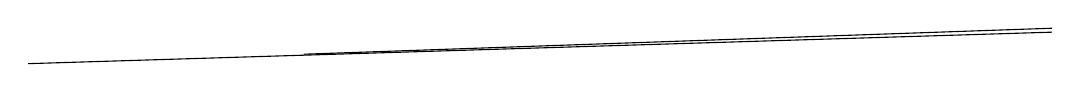
\begin{tikzpicture}\draw (0,0)--(13,.4);\draw (3.5,.12)--(13,.45);\end{tikzpicture}}

Supposons $W$ non singulière, i.e. $\mathring M$ non singulière, i.e. $\mathring P$ non singulière. Alors on a un isomorphisme
\[
\mathbb R(\Gamma,\pi)_!(\mathring M)\simeq\mathbb R\operatorname{Hom}_{\Lambda}\left(\underset{\substack{\Vert\\\mathbb R(\Gamma,\pi)(M)}}{K^\bullet},\Lambda\right)[-2n]
\]
et la flèche verticale de \textcircled{a} est une flèche
\diagram{\begin{tikzcd}[column sep=large]
\boxed{u:\ \mathbb R\operatorname{Hom}_{\Lambda}(K^\bullet,\Lambda)[-2n]\longrightarrow K^\bullet}&\text{dans }\mathrm D(\Lambda[\pi])
\end{tikzcd}}
i.e. un élément de
\[
\deleted{\unsure{\mathbb R\Gamma(\Lambda)}}\ H^{2n}(K^\bullet\overset{\mathrm L}{\otimes}_{\Lambda}K^\bullet)
\]
La donnée fondamentale \textcircled{a} devient
\textcircled{a'}
\diagram{\begin{tikzcd}[row sep=large,column sep=large]
& L^{\bullet\,\mathrm{triv}} \arrow[dl,"\rho'"']\\
\mathbb R\operatorname{Hom}_{\Lambda}(K^\bullet,\Lambda)[-2n] \arrow[r,very thick] &K^\bullet \arrow[u,"\rho"]
\end{tikzcd}}
\margin{$K^\bullet\in\operatorname{ob}\mathrm D(\Lambda[\pi])$;\par
$L^\bullet\in\operatorname{ob}\mathrm D(\Lambda)$\par
$K^\bullet$ parfait rel. à $\Lambda$}

En fait, $\rho$ et $\rho'$ \uuline{sont transposés} \uline{l'un de l'autre} (signe ?)
\mspage{21}
\scanpage{23}
\mspage{22}
\figure{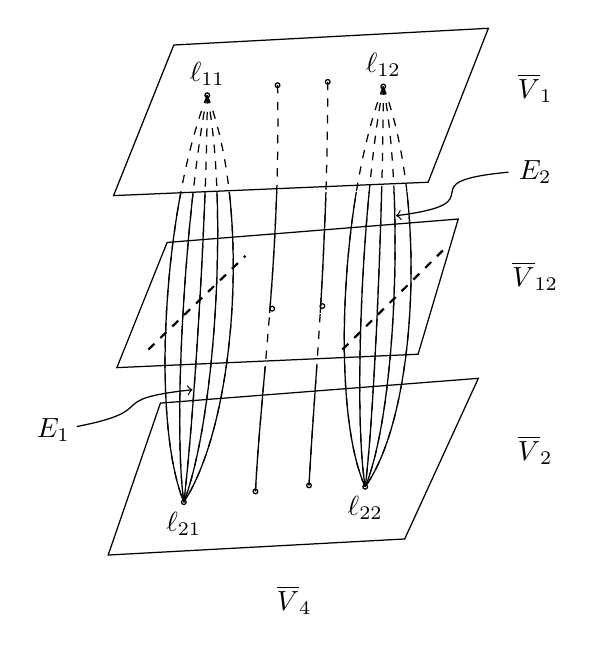
\begin{tikzpicture}[scale=.85,line width=.45pt]
\draw (.9,8.1)--(5.6,8.35)--(4.7,6.05)--(0,5.85)--cycle;
\draw (.8,5.15)--(5.15,5.5)--(4.55,3.48)--(.05,3.28)--cycle;
\draw (.7,2.75)--(5.45,3.12)--(4.35,.72)--(-.08,.48)--cycle;
\foreach \d in {-.65,-.32,0,.32,.65}{
\draw[dashed] (1.4,7.35)..controls ({1.4+\d},5.7) and ({1.2+\d},2.5)..(1.05,1.27);
\draw[dashed] (4.03,7.48)..controls ({4.03+\d},5.8) and ({3.9+\d},2.6)..(3.76,1.5);
\begin{scope}\clip (-1,3.28) rectangle (6,5.9);
\draw (1.4,7.35)..controls ({1.4+\d},5.7) and ({1.2+\d},2.5)..(1.05,1.27);
\draw (4.03,7.48)..controls ({4.03+\d},5.8) and ({3.9+\d},2.6)..(3.76,1.5);
\end{scope}
\begin{scope}\clip (-1,.4) rectangle (6,3.3);
\draw (1.4,7.35)..controls ({1.4+\d},5.7) and ({1.2+\d},2.5)..(1.05,1.27);
\draw (4.03,7.48)..controls ({4.03+\d},5.8) and ({3.9+\d},2.6)..(3.76,1.5);
\end{scope}
}
\draw[dashed] (2.45,7.5)..controls (2.5,5) and (2.2,3)..(2.12,1.43);
\draw[dashed] (3.2,7.55)..controls (3.2,5) and (3,3)..(2.92,1.52);
\begin{scope}\clip (0,4.1) rectangle (5,5.9);
\draw (2.45,7.5)..controls (2.5,5) and (2.2,3)..(2.12,1.43);
\draw (3.2,7.55)..controls (3.2,5) and (3,3)..(2.92,1.52);
\end{scope}
\begin{scope}\clip (0,1) rectangle (5,3.3);
\draw (2.45,7.5)..controls (2.5,5) and (2.2,3)..(2.12,1.43);
\draw (3.2,7.55)..controls (3.2,5) and (3,3)..(2.92,1.52);
\end{scope}
\draw[dashed,line width=.8pt] (.52,3.55)--(1.97,4.95);
\draw[dashed,line width=.8pt] (3.42,3.55)--(4.95,5.06);
\foreach \p in {(1.4,7.35),(4.03,7.48),(2.45,7.5),(3.2,7.55),(2.37,4.16),(3.12,4.2),(1.05,1.27),(2.12,1.43),(2.92,1.52),(3.76,1.5)}{\draw \p circle (.035);}
\node[above] at (1.4,7.35) {$\ell_{11}$};\node[above] at (4.03,7.48) {$\ell_{12}$};
\node[below] at (1.05,1.27) {$\ell_{21}$};\node[below] at (3.76,1.5) {$\ell_{22}$};
\node at (6.3,7.45) {$\overline V_1$};\node at (6.3,4.65) {$\overline V_{12}$};\node at (6.3,2.05) {$\overline V_2$};
\node at (2.7,-.2) {$\overline V_4$};
\node at (-.9,2.35) {$E_1$};\draw[->] (-.55,2.4)..controls (.75,2.65) and (-.2,2.8)..(1.18,2.95);
\node at (6.3,6.2) {$E_2$};\draw[->] (5.9,6.2)..controls (4.3,6.05) and (5.8,5.75)..(4.22,5.55);
\end{tikzpicture}}

\figure{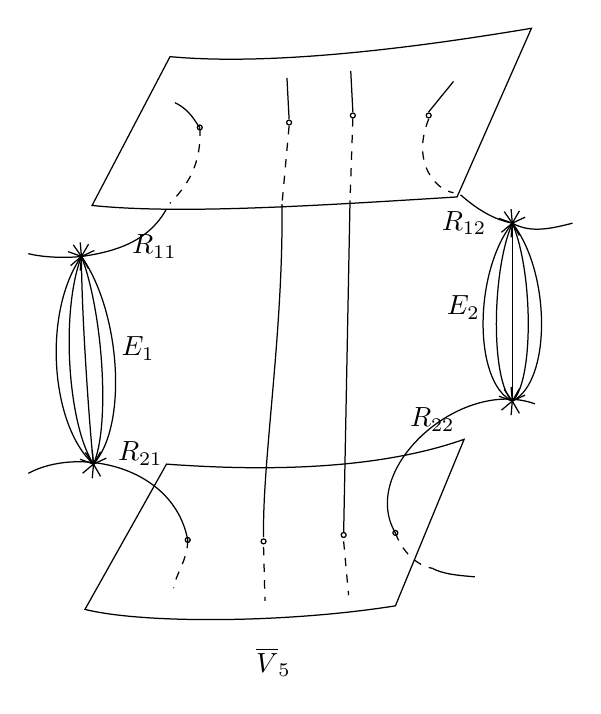
\begin{tikzpicture}[scale=.9,line width=.45pt]
\draw (.5,7.8)..controls (2.1,7.65) and (4.4,8)..(5.6,8.2)--(4.55,5.82)..controls (2.6,5.7) and (.65,5.57)..(-.6,5.7)--cycle;
\draw (.45,2.05)..controls (2.5,1.9) and (3.8,2.1)..(4.65,2.4)--(3.68,.05)..controls (2.1,-.2) and (.1,-.2)..(-.7,0)--cycle;
\draw (.57,7.15)..controls (.8,7.04) and (.87,6.85)..(.92,6.8);
\draw[dashed] (.92,6.8)..controls (.95,6.25) and (.72,5.96)..(.5,5.73);
\draw (.45,5.65)..controls (.2,5.2) and (-.25,5.05)..(-.75,4.98)..controls (-1.05,4.95) and (-1.35,4.98)..(-1.5,5.02);
\draw (4.5,7.45)--(4.15,7.02);
\draw[dashed] (4.15,6.92)..controls (3.9,6.3) and (4.25,5.92)..(4.5,5.88);
\draw (4.6,5.85)..controls (4.85,5.63) and (5.08,5.5)..(5.33,5.45)..controls (5.6,5.3) and (5.9,5.38)..(6.18,5.45);
\foreach \d in {-.55,-.3,0,.3,.55}{
\draw (-.75,4.98)..controls ({-.75+\d},4.2) and ({-.64+\d},2.6)..(-.58,2.05);
\draw (5.33,5.45)..controls ({5.33+\d},4.75) and ({5.33+\d},3.2)..(5.33,2.94);
}
\draw (-1.5,1.92)..controls (-.8,2.3) and (.55,2.03)..(.75,.98);
\draw[dashed] (.75,.98)..controls (.75,.7) and (.58,.5)..(.55,.3);
\draw (5.65,2.9)..controls (4.6,3.28) and (3.15,1.98)..(3.68,1.08);
\draw[dashed] (3.68,1.08)..controls (3.8,.75) and (4.05,.6)..(4.2,.58);
\draw (4.2,.58)..controls (4.35,.5) and (4.55,.48)..(4.8,.46);
\draw (2.15,7.5)--(2.18,6.92);\draw[dashed] (2.18,6.82)--(2.08,5.72);
\draw (2.08,5.72)..controls (2.1,3.9) and (1.8,2.1)..(1.82,1.02);\draw[dashed] (1.82,.88)--(1.84,.12);
\draw (3.05,7.6)--(3.08,7.02);\draw[dashed] (3.08,6.93)--(3.04,5.77);
\draw (3.04,5.77)--(2.95,1.08);\draw[dashed] (2.95,.96)--(3.02,.2);
\foreach \p in {(.92,6.8),(2.18,6.87),(3.08,6.97),(4.15,6.97),(.75,.98),(1.82,.96),(2.95,1.05),(3.68,1.08)}{\draw \p circle (.035);}
\foreach \x/\y in {-.75/4.98,-.58/2.05,5.33/5.45,5.33/2.94}{\foreach \ang in {25,60,95,125,160,220,265,300}{\draw (\x,\y)--++(\ang:.2);}}
\node at (.28,5.12) {$R_{11}$};\node at (4.65,5.45) {$R_{12}$};\node at (.08,2.2) {$R_{21}$};\node at (4.2,2.68) {$R_{22}$};
\node at (.05,3.68) {$E_1$};\node at (4.64,4.26) {$E_2$};\node at (1.96,-.75) {$\overline V_5$};
\end{tikzpicture}}

\uline{Figure 8}
\scanpage{24}
donc le triangle \textcircled{a} ou \textcircled{a'} apparaît comme \uline{autotransposé}.

Appliquons le foncteur oubli, on trouve
\textcircled{c'}
\diagram{\begin{tikzcd}[row sep=large,column sep=large]
&L^\bullet\simeq\mathbb R\Gamma(W_0) \arrow[dl]\\
\mathbb R\operatorname{Hom}_{\Lambda}(K^{\bullet\mathrm{oub}},\Lambda)[-2n] \arrow[r] \arrow[d,equal] &K^{\bullet\mathrm{oub}}\simeq\mathbb R\Gamma(M) \arrow[u]\\
\mathbb R\Gamma_!(\mathring M)&
\end{tikzcd}}
\margin{\uline{dire que c'est encore un triangle autotransposé}}

Appliquons $\mathbb R\Gamma^\pi$, on trouve
\margin{[\uline{expliquer} comment ?]}
\textcircled{b'}
\margin{\deleted{\unsure{1}}}
\diagram{\begin{tikzcd}[row sep=large,column sep=large]
&L^\bullet\overset{\mathrm L}{\otimes}_{\Lambda}\mathbb R\Gamma(S^1)\simeq L^\bullet\times L^\bullet[-1]\simeq\unsure{I|l} \arrow[dl,"(\alpha',\beta')"']\\
\mathbb R\operatorname{Hom}_{\Lambda}(K^{\bullet\pi},\Lambda)[-2n-1] \arrow[r,very thick] \arrow[d,equal]&K^{\bullet\pi}\simeq\mathbb R\Gamma(P)\simeq\mathbb R\Gamma(W-W_0) \arrow[u,"(\alpha,\beta)",very thick]\\
\mathbb R\Gamma_!(\mathring P)\simeq\mathbb R\Gamma_!(W-W_0)&
\end{tikzcd}}
\margin{\fbox{\begin{minipage}{.33\linewidth}vérifier la commutation de $\mathbb R\Gamma^\pi$ à $\mathbb R\operatorname{Hom}_{\Lambda}(-,\Lambda)=(-)^\vee$\end{minipage}}}
\margin{(triangle autotransposé)}

\deleted{\unsure{Et les} \uline{triangles} \textcircled{d} et \textcircled{e} \uline{deviennent chacun}}

Comme nouvelle \deleted{\unsure{donnée}} \inserted{structure}, ce triangle introduit
\deleted{\diagram{\begin{tikzcd}
u_1:\ \mathbb R\operatorname{Hom}_{\Lambda}(K^\bullet,\Lambda)[-2n-1] \arrow[r] &\unsure{H|K}
\end{tikzcd}}}
\diagram{\begin{tikzcd}[column sep=large]
\boxed{u_1:\ \mathbb R\Gamma(W-W_0)^\vee[-2n-1]\mathbin{-}\mathbb R\Gamma(W-W_0)}
\end{tikzcd}}
et des accouplements
\diagram{\begin{tikzcd}
\boxed{\begin{gathered}
\lambda:\ \mathbb R\Gamma(W_0)\times\mathbb R\Gamma(W-W_0)\mathbin{-}\Lambda[-2n]\\
\mu:\ \mathbb R\Gamma(W_0)\times\mathbb R\Gamma(W-W_0)\mathbin{-}\Lambda[-(2n-1)]
\end{gathered}}
\end{tikzcd}}
\diagram{\begin{tikzcd}
\lambda:\ H^{\deleted{i}\inserted{2n-i}}(W_0)\times H^{\deleted{\unsure{2n-i}}\inserted{i}}(W-W_0) \arrow[r] &\Lambda\\
\mu:\ H^{\deleted{i}\inserted{2n-1-i}}(W_0)\times H^{\deleted{\unsure{2n-1-i}}\inserted{i}}(W-W_0) \arrow[r,dash] &\Lambda
\end{tikzcd}}
i.e.
\diagram{\begin{tikzcd}
\lambda':\ H^{\deleted{\unsure{2n-}}i}(W-W_0) \arrow[r]&H^{i-1}(W_0)&\text{je dis que c'est }\deleted{\unsure{le}}\ \beta\\
\mu':\ H^i(W-W_0) \arrow[r]&H^i(W_0)&\text{je dis que c'est }\alpha
\end{tikzcd}}
\mspage{23}
\scanpage{25}
\mspage{24}
\begin{center}-4.14-\end{center}

of $\overline V_4$ are precisely the four lines $\ell_{ij}\subset\overline V_i\subset\overline V_4$, and $H_4$ passes through all of them. A local computation shows that these singularities are all resolved on $\overline V_5$, and each line $\ell_{ij}$ is blown up into a ruled surface $R_{ij}$. Moreover, the action of $\mathbb G_m$ lifts to $\overline V_5$, since $H_4$ is invariant under $\mathbb G_m$, and $\mathbb G_m$ acts non-trivially on the ruled surface $R_{ij}$ with orbit space $\ell_{ij}$. Finally, define $V_5$ to be the opensubset of $\overline V_5$ obtained by removing:
\margin{$\unsure{\sim\sim}$}

a) the proper transforms of $\overline V_1$, $\overline V_2$ ;

b) the proper transforms on $\overline V_5$ of the divisors $E_1$ and $E_2$ on $\overline V_4$; where $E_1$ is the locus of lines joining $\ell_{11}$ and $\ell_{21}$, and $E_2$ is the locus of lines joining $\ell_{12}$ and $\ell_{22}$ ;

c) $R_{12}$ and $R_{21}$.

A rather conceptualized ``picture'' of $V_5$ is given in Figure 8.

It is clear that $V_5$ is invariant under the action of $\mathbb G_m$, and that $V_3$ is a geometric quotient of $V_5$ by $\mathbb G_m$: for $V_5$ is the union of the lines joining biregularly corresponding points of $V_1$ and $V_2$, plus the lines of $R_{11}$ and of $R_{22}$.

Note also that the automorphism $\sigma_{\unsure{o|0}}$ can be carried along:

i) $\sigma$ lifts to an isomorphism $\overline V_1\longrightarrow\overline V_2$ ; ii) if the embeddings $\overline V_i\subset\mathbb P_{n_i}$ are chosen suitably, $\sigma$ extends to an isomorphism $\mathbb P_{n_1}\longrightarrow\mathbb P_{n_2}$ ; iii) this isomorphism extends to an automorphism of $\mathbb P_{n_1+n_2+1}$ of order 2 satisfying $\sigma.\alpha.\sigma^{-1}=\unsure{-}\alpha^{-1}$, for $\alpha\in(\unsure{\overline{\mathbb G}_m|\mathbb G_m})$ acting on $\mathbb P_{n_1+n_2+1}$ ; iv) $\sigma$ takes $\overline V_4$ into itself, and $H_4$ into itself, hence $\sigma$ lifts to a morphism $\sigma:\overline V_5\longrightarrow\overline V_5$; v) this $\sigma$ carries
\scanpage{26}
On obtient donc deux données \unsure{remarquables}, savoir $u$ et
\[ L^{\bullet\,\mathrm{triv}}\times K^\bullet\longrightarrow\Lambda[-2n+1] \]
i.e.
\[\boxed{\text{\unsure{accoupl.}}\quad \mathbb R\Gamma(W_0)^{\mathrm{triv}}\times\mathbb R(\Gamma,\pi)(M)\longrightarrow\Lambda[-(2n-1)]}\]
i.e.
\diagram{\begin{tikzcd}[column sep=large]
\mathbb R(\Gamma,\pi)(M)\arrow[r]&\mathbb R\Gamma(W_0)^\vee[-(2n-1)]^{\mathrm{triv}}\arrow[r,"\sim"{description},equals]&\mathbb R\Gamma(W_0)^{\mathrm{triv}}\\
&\text{p.r. à }\Lambda\arrow[u,no head,bend right=25]&\text{dualité de }W_0\arrow[u,no head]
\end{tikzcd}}

\uline{Enfin}, \uline{les triangles} $\textcircled{d}$ \uline{et} $\textcircled{e}$ \uline{sont transposés}

\uline{NB} En prenant des coefficients généraux, loc. triviaux au voisinage de \deleted{\unsure{\(\partial\)}} $W_0$, on trouve que, passant de ces coefficients à des coefficients ``duaux'', \deleted{\unsure{les preuves}} sous hyp. de \deleted{singularité} non singularité sur $W$, les suites ex.tes du type $\textcircled{a},\textcircled{b},\textcircled{c}$ sont \unsure{transposées} de suites exactes \uline{du $=$ type}, et les suites ex.tes du type $\textcircled{e}$ sont transposées de celles du type $\textcircled{d}$.

\figure{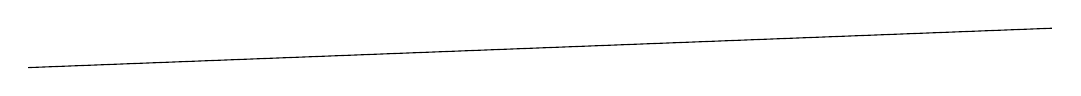
\begin{tikzpicture}\draw (0,0)--(13,0.5);\end{tikzpicture}}
\margin{\unsure{plus bas}}
Supposons que $W$ \uline{soit une} \uline{sphère} \inserted{(de dim $2n+1$)}. Alors la suite exact\unsure{e} \deleted{\unsure{d)}} \uline{déduite} de $d)$
\[\cdots\longrightarrow H^{i-2}(W_0)\longrightarrow H^i(W)\longrightarrow H^i(W-W_0)\longrightarrow H^{i-1}(W_0)\longrightarrow H^{i+1}(W)\]
montre ceci :

$a)$ Si $i,i+1\ne0,2n+1$, \inserted{i.e. $i\ne0,2n,2n+1$} \inserted{(en fait, en vertu de $b)$, il suffit que $i\ne0,2n$)} alors
\[H^i(W-W_0)\xrightarrow{\sim}H^{i-1}(W_0)\]
\deleted{$b)\quad \cdots\longrightarrow H^{2n}(W-W_0)\longrightarrow H^{2n-1}(W_0)\longrightarrow\Lambda\longrightarrow \unsure{0}\,\unsure{H^{2n+1}(W-W_0)}\longrightarrow \unsure{0}\,H^{2n}(W_0)\longrightarrow0$}
\deleted{\[H^{2n+1}(W-W_0)\simeq H^{2n}(W_0)\simeq0\]}
\mspage{25}
\scanpage{27}
\begin{center}-4.13-\end{center}
This is the first step of the construction. Now fix some projection embeddings of $\overline V_1$ and $\overline V_2$, say $\overline V_1\subset\mathbb P_{n_1}$, $\overline V_2\subset\mathbb P_{n_2}$. Embed $\mathbb P_{n_1}$ and $\mathbb P_{n_2}$ as disjoint linear subspaces of $\mathbb P_{n_1+n_2+1}$, and consider the two subvarieties $\overline V_i\subset\mathbb P_{n_1+n_2+1}$. Let $\overline V_4$ be the locus of lines in $\mathbb P_{n_1+n_2+1}$ joining birationally corresponding points of $\overline V_1$ and $\overline V_2$ (cf. Figure 8, where all dimensions have been lowered by one). Now the group $\mathbb G_m$ operates in a natural way on $\mathbb P_{n_1+n_2+1}$ so as to leave $\mathbb P_{n_1}$ and $\mathbb P_{n_2}$ pointwise fixed. This induces an action of $\mathbb G_m$ on $\overline V_4$, leaving the subvarieties $\overline V_1$ and $\overline V_2$ pointwise fixed. Now let $\phi:\overline V_4\longrightarrow V_o$ be the natural projection. Also introduce for convenience a hyperplane $H_o\subset V_o$ through $P_1$ and $P_2$ and left fixed by $\sigma_o$ (there are, in fact, exactly two such hyperplanes). Let $H_4$ be its proper inverse image under $\phi$, i.e., the irreducible subvariety of $\overline V_4$ that dominates $H_o$ and is a component of $\phi^{-1}(H_o)$. Let $I\subset\uline{o}_{\overline V_4}$ be the sheaf of ideals vanishing on $H_4$. Define $\overline V_5$ as the I-transform of $\overline V_4$ (cf. EGA 2, \S8). We wish to describe explicitly the structure of $\overline V_5$. Let $\overline V_{12}$ be the birational joint of $\overline V_1$ and $\overline V_2$, be $v_j$ be the m-adic valuation of the function field $k(V_o)$ centered at $P_j$, and let $\ell_{ij}$ be the center of $v_j$ on $\overline V_i$. Then one verifies readily that $\ell_{ij}$ are lines on $\overline V_i$ and that $\overline V_{12}$ is obtained from $\overline V_i$ by blowing up $\ell_{i1}$ and $\ell_{i2}$. But $\overline V_4$ is essentially a (twisted) product of $(\mathbb P_1-2\text{ points})$ by $\overline V_{12}$, with $\overline V_1$ and $\overline V_2$ at the two ends. $\overline V_5$ differs from $\overline V_4$ only at points of $H_4$ which are singular on $\overline V_4$. In fact, the singularities
\mspage{26}
\scanpage{28}
$b)$ La portion de suite exacte
\diagram{\begin{tikzcd}[column sep=small,row sep=small]
H^{2n}(W)\arrow[r,no head]\arrow[d,equals]&H^{2n}(W-W_0)\arrow[r,no head,"\mathrm{inj}"]&H^{2n-1}(W_0)\arrow[r,"\mathrm{surj}"]\arrow[d,equals]&H^{2n+1}(W)\arrow[r,no head]\arrow[d,equals]&H^{2n+1}(W-W_0)\arrow[r,no head]\arrow[d,equals]&H^{2n}(W_0)\arrow[r]\arrow[d,equals]&0\\
0&&\Lambda&\Lambda&0&0
\end{tikzcd}}
\margin{si $W_0$ est connexe, tjrs le cas si $n\ge2$}
donne
\[\left\{\begin{gathered}
\boxed{H^{2n}(W-W_0)}=H^{2n+1}(W-W_0)=0\\
\underset{\Vert\;\Lambda}{H^{2n-1}(W_0)}\simeq\underset{\Vert\;\Lambda}{H^{2n+1}(W)}
\end{gathered}\right.\]
\margin{\unsure{conclusion visible de} Lefschetz affine local plus bas}
\margin{\uline{NB} $H^i(W_0)=0$ sauf si $i\in[0,2n-1]$. $H^\bullet(W_0)$ satisfait dualité de Poincaré}
\margin{\deleted{\unsure{supposons}}}
\margin{\uline{NB} $W$ sph. coh. $\Longleftrightarrow$ \deleted{\unsure{\(W-W_0\)}}
\[\left\{\begin{gathered}H^i(W-W_0)\xrightarrow{\sim}H^{i-1}(W_0)\quad\text{si }i\ne0,2n\\
\text{et }H^{2n}(\deleted{W}\unsure{W}-W_0)\hookrightarrow H^{2n-1}(W_0)\end{gathered}\right.\]
[Si \deleted{\unsure{de plus}} $W_0$ connexe, cela équivaut à $H^{2n}(W-W_0)=0$]
Si $n\ge2$, et $W$ non-singulier, il \uuline{f.} que $H^{2n}(W-W_0)=0$, $W_0$ connexe}

\figure{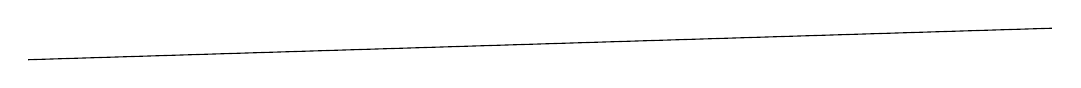
\begin{tikzpicture}\draw (0,0)--(13,0.4);\end{tikzpicture}}
Supposons que $X$ soit régulier en $\deleted{X}x$. Alors on a, par

\uline{Lefschetz local} :
\[\left\{\begin{array}{lll}
H^i(W)\longrightarrow H^i(W_0)&\text{un isom pour}&i\le n-\unsure{2|1}\\
&\text{un mono pour}&i=n\deleted{\unsure{-2}}-1
\end{array}\right.\]
\deleted{Donc si $W$ est une sphère,}

\deleted{Par la suite exacte associée à $e)$, cela signifie}
\inserted{\unsure{dualité cela s'interprète}}
\[\left\{\begin{array}{lll}
H^i_{\unsure{!}}(W_0)\longrightarrow H^{i+2}(W)&\text{un isom si}&i\ge n+\unsure{1}\\
&\text{un épim si}&i\unsure{\ge|=}n\deleted{\unsure{+1}}
\end{array}\right.\]
donc la connaissance de la cohomologie de $W$ implique celle de la cohomologie de $W_0$, sauf en les deux dimensions \deleted{$n-1,n$}\inserted{$H^{n-1}(W_0),H^n(W_0)$} (complémentaires, i.e. où les cohomologies sont duales pour $W_0$).

On peut dire aussi que l'on a
\[\left[\begin{array}{ll}H^i(W-W_0)=0&\text{si }i>n+1\\[-.4em]\quad\Vert&\\[-.4em]\quad H^i(P)&\end{array}\right.\]
\mspage{27}
\scanpage{29}
\begin{center}-4.12-\end{center}
The first example is due to Nagata [27]. Here $\mathrm{SL}(3)$ is acting on an open set $U$ in $|5H|$, as in \S2. The geometric points of $U$ are precisely those plane quintic curves $C$ such that:

\begin{enumerate}
\item[i)] $C$ has no 4th order points,
\item[ii)] $C$ has no triple points, with tangent cone one line, and that line having 5-fold contact with $C$,
\item[iii)] $C$ has no triple points, consisting of a simple branch, and a tacnode,
\item[iv)] no component of $C$ is a line.
\end{enumerate}
Nagata has proven that $\mathrm{SL}(3)$ acts properly on $U$. But from the results of \S2, it follows that no geometric quotient of $U$ by $\mathrm{SL}(3)$ exists.

The second example is based on an example of Hironaka [15]. Let $V_o$ be $\mathbb P_3$, and let $\gamma_1$, $\gamma_2$ be two conics in $V_o$, intersecting normally in exactly two points $P_1$ and $P_2$. Following Hironaka, construct $\overline V_i$, for $i=1$ and $2$, by (a) blowing up $\gamma_i$ in $V_o$; (b) blowing up $\gamma_{3-i}$ in the result (cf. Figure 7). Let $V_i$ be the open set in $\overline V_i$ of points lying over $(V_o-P_{3-i})$. Then by patching $V_1$ and $V_2$, we obtain a single non-projective variety $V_3$ in which, over $P_1$ and $P_2$ the two curves $\gamma_1$ and $\gamma_2$ have been blown up in opposite orders! Now let $\sigma_o:V_o\longrightarrow V_o$ be a projective transformation of order 2 which permutes $P_1$ and $P_2$, and also $\gamma_1$ and $\gamma_2$. Then $\sigma_o$ induces an automorphism of $V_3$ of order 2. Hironaka has shown that there is no geometric quotient of $V_3$ by the group $\mathbb Z_2=\{1,\sigma\}$, although of course there is an analytic space $[V_3/\mathrm{mod}\,\mathbb Z_2]$.
\mspage{28}
\scanpage{30}
Revenant au cas $W$ une sphère, on trouve
\[\left\{\begin{array}{ll}H^i(W-W_0)=0&\text{si }i>n+1\\H^i(W_0)=0&\text{si }i\ne n-1,n,0,2n-1\end{array}\right.\]
\margin{[en fait, si $i\ne\deleted{\unsure{n,n+1}}\deleted{\unsure{]}}0,1,n,n+1$]}
\margin{(d'abord si $i\ge n+1$ et $i\ne2n-1$, puis le reste par dualité]}

La suite exacte associée à $d)$ est triviale, sauf la portion
\[\left\{\begin{gathered}
0\unsure{\mathbin{-}|\longrightarrow}H^0(W)\longrightarrow H^0(W-W_0)\longrightarrow0\\
0\unsure{\mathbin{-}|\longrightarrow}H^n(W-W_0)\longrightarrow H^{n-1}(W_0)\longrightarrow0\\
0\unsure{\mathbin{-}|\longrightarrow}H^{n+1}(W-W_0)\longrightarrow H^n(W_0)\xrightarrow[\text{si }n\ne1]{}0\\
0\longrightarrow H^{2n-1}(W_0)\longrightarrow H^{2n+1}(W)\longrightarrow0
\end{gathered}\right.\]
\[0\unsure{\mathbin{-}|\longrightarrow}H^1(W-W_0)\longrightarrow H^0(W_0)\longrightarrow0\]
\deleted{\[\unsure{n+1\ne2n+1}\]}
\deleted{\[n+2\ne2n+1\]}

[Si $n=1$, on trouve
\[\begin{gathered}
0\longrightarrow H^0(W)\xrightarrow{\sim}H^0(W-W_0)\mathbin{-}0\\
0\longrightarrow H^1(W-W_0)\longrightarrow H^0(W_0\deleted{\unsure{\Lambda}})\mathbin{-}0\\
0\unsure{\mathbin{-}|\longrightarrow}H^2(W-W_0)\longrightarrow H^1(W_0)\longrightarrow\underset{\Vert\;\Lambda}{H^3(W)}\longrightarrow0
\end{gathered}\]
]
\figure{\begin{tikzpicture}\draw (0,0)--(13,0.6);\end{tikzpicture}}
Notons que, par \unsure{passage} à la limite, \deleted{\unsure{les les}} les relations
\[H^i(W\unsure{-}W_0,\Lambda)=0\quad\text{pour }i>n\deleted{\unsure{+1}}\]
donnent
\[\boxed{H^i(M,\Lambda)=0\quad\text{si }i>n\deleted{\unsure{+1}}}\]
\margin{[\unsure{Indépendt} du fait que $W$ non singulier] \inserted{et \unsure{même} que $W_0$ non singulier}}

La suite exacte relative (si $W$ non singulier)
\[\mathbin{-}\unsure{\mathbin{-}|\longrightarrow}H^{\unsure{2n-i}}(M)^\vee\longrightarrow H^i(M)\unsure{\mathbin{-}|\longrightarrow}H^i(W_0)\longrightarrow H^{2n-i\unsure{+1|-1}}(M)^\vee\longrightarrow H^{i+1}(M)\longrightarrow H^{\unsure{i+1}}(W_0)\]
montre donc que

\deleted{Si $i>n+1$}
\mspage{29}
\scanpage{31}
\mspage{30}
\begin{center}-4.11-\end{center}
Now consider the skeleton $\Delta(T)$ in $\Delta(\overline{\mathrm{SL}(3)})$. It can be represented as the set of points on the circle
\[\begin{gathered}r_o+r_1+r_2=0\\r_o^2+r_1^2+r_2^2=6\end{gathered}\]
where the ratios of the $r_i$'s are rational. If $\ell_i$ is the line in $\mathbb P_2$ given by $x_i=0$, and if $P_i$ is the point in $\mathbb P_2$ with coordinates $x_j=\delta_{ij}$, then proceeding around this circle, the parabolic subgroups correspond to flags as indicated in Diagram 5. Furthermore, for a 1-PS $\lambda$ of $T$ as above, put:
\[\Vert\lambda\Vert=\sqrt{(r_o^2+r_1^2+r_2^2)/6}\]
The resulting function $\unsure{\nu|v}^{o(1)}(C,*)$ is indicated in Diagram 6, for some simple curves $C$.

\fbox{\S3.} In this section, we shall consider counter-examples. We would like to show how the reductive groups $\mathrm{SL}(n)$ can operate properly on \uline{quasi-projective} schemes $X$, simple over $\unsure{\mathbb Q|\mathbb C}$, but where there is \uline{no} geometric quotient of $X$ by $\mathrm{SL}(n)$; i.e, by Converse 1.12 and Proposition 0.7, there is no $L$ in $\mathrm{Pic}^G(X)$ such that $X=X^s(L)$. It should be emphasized that in any such case, there is an analytic space which is a quotient of the analytic space defined by $X$,by the analytic group $\mathrm{SL}(n)$: cf. Palais [31]. The moral of these examples is that the concept of stable points is purely algebraic, and not topological.
\scanpage{32}
\deleted{En d'autres termes, le \unsure{triangle}}
\deleted{\[H^i(W_0)=0\quad\text{si }i\ne\unsure{i|1}\]}
\deleted{\[\begin{gathered}\unsure{i=n+1}\\\unsure{2n-i=n-1}\end{gathered}\]}
\margin{\uline{\unsure{intéressant}}}
\[\left\{\begin{array}{ll}
H^i(W_0)\xrightarrow{\sim}H^{2n-i-1}(M)^\vee&\text{si }i\ge n+\unsure{1|2}\\
\boxed{H^i(M)\xrightarrow{\sim}H^i(W_0)}&\text{si }i\le n-2
\end{array}\right.\]
\margin{(épim si $i=\unsure{n-1|n}$)}
\margin{(donc $2n-i-1\le n-3$)}
\margin{(mono si $i=n-1$)}
Donc $H^{\unsure{q|*}}(M)$ est connu en termes de $H^{\unsure{q|*}}(W_0)$ sauf aux dimensions \deleted{$\unsure{n}$} $n-1,n$, \deleted{$\unsure{n}$}, où on a la suite exacte
\diagram{\begin{tikzcd}[column sep=small,row sep=large]
\deleted{0}\arrow[r]&\deleted{H^{n-2}(M)}\arrow[r]&\deleted{H^{n-2}(W_0)}\arrow[r]&\deleted{H^{\unsure{2n+1|n+1}}(M)^\vee}\inserted{0}\arrow[r]&H^{n-1}(M)\arrow[r]&H^{n-1}(W_0)\arrow[r,"\mathrm{surj}"]\arrow[d,no head,"\deleted{\unsure{\simeq}}"]&H^{\unsure{n}}(M)^\vee\arrow[d]\\
\deleted{0}&\deleted{H^{n-2}(M)^\vee}\arrow[l]&\deleted{H^{n+1}(W_0)}\arrow[l]&\deleted{H^{n+1}(M)}\inserted{0}\arrow[l]&H^{n-1}(M)^\vee\arrow[l]&H^n(W_0)\arrow[l]&H^n(M)\arrow[l,"\deleted{\unsure{\rho}}"]
\end{tikzcd}}

Supposons maintenant que $W$ \unsure{est} la sphère topologique. Alors on a vu que $H^i(W_0)=0$ si $i\ne0,n-1,n,2n-1$.

\uuline{Si donc} \textcircled{$n\ge3$}, on trouve aussi \uline{$H^{\inserted{i}\deleted{\unsure{n-2}}}(M)=0$}, \deleted{$\unsure{H^{n-2}(M)=0}$}
\inserted{si $i\ne0,n-1,n$, \deleted{$\unsure{2n}$}}

\deleted{et la suite exacte précédente devient}
\deleted{\diagram{\begin{tikzcd}[column sep=small,row sep=large]
&+&-&+&-\\
0\arrow[r]&H^{\unsure{n-1|n+1}}(M)^\vee\arrow[r,"u"]&H^{n-1}(M)\arrow[r]&H^{n-1}(W_0)\arrow[r]&H^n(M)^\vee\arrow[d,very thick]\\
0&H^{n+1}(M)\arrow[l]&H^{n-1}(M)^\vee\arrow[l,"u'"']&H^n(W_0)\arrow[l]&H^n(M)\arrow[l]\\
&-&+&-&+\\
&\unsure{H}
\end{tikzcd}}}
\mspage{31}
\scanpage{33}
\mspage{32}
\figure{\begin{tikzpicture}[x=.01cm,y=-.01cm]
\draw[dash pattern=on 32pt off 24pt] (310,265) ellipse (310 and 265);
\draw (130,170).. controls (160,215) and (235,265)..(300,295).. controls (385,334) and (440,323)..(530,320);
\draw (373,130)..controls (330,195) and (307,270)..(300,295)..controls (281,365) and (276,408)..(284,454);
\draw (300,295) circle (6);
\node at (270,250) {$P_1$};\node at (245,445) {$\gamma_1$};\node at (520,360) {$\gamma_2$};
\end{tikzpicture}}
\figure{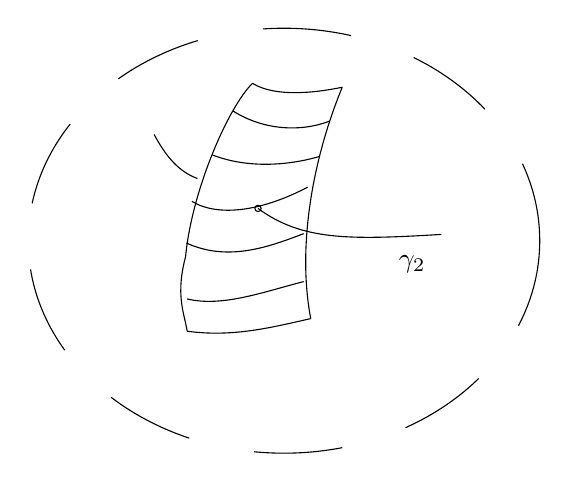
\begin{tikzpicture}[x=.01cm,y=-.01cm]
\draw[dash pattern=on 32pt off 24pt] (325,270) ellipse (325 and 270);
\draw (285,70)..controls (255,99) and (208,205)..(200,290)..controls (187,339) and (198,361)..(202,385);
\draw (399,75)..controls (360,170) and (342,280)..(359,369);
\draw (285,70)..controls (314,88) and (365,82)..(399,75);
\draw (202,385)..controls (260,393) and (310,380)..(359,369);
\draw (260,105)..controls (299,130) and (347,132)..(383,118);
\draw (234,161)..controls (275,177) and (325,176)..(370,163);
\draw (208,220)..controls (241,240) and (296,233)..(355,202);
\draw (201,273)..controls (252,296) and (301,280)..(350,261);
\draw (202,344)..controls (247,355) and (302,334)..(350,322);
\draw (160,135)..controls (175,163) and (191,182)..(215,191);
\draw (292,229)..controls (348,270) and (408,269)..(525,262);
\draw (292,229) circle (4);\node at (488,300) {$\gamma_2$};
\end{tikzpicture}}
\figure{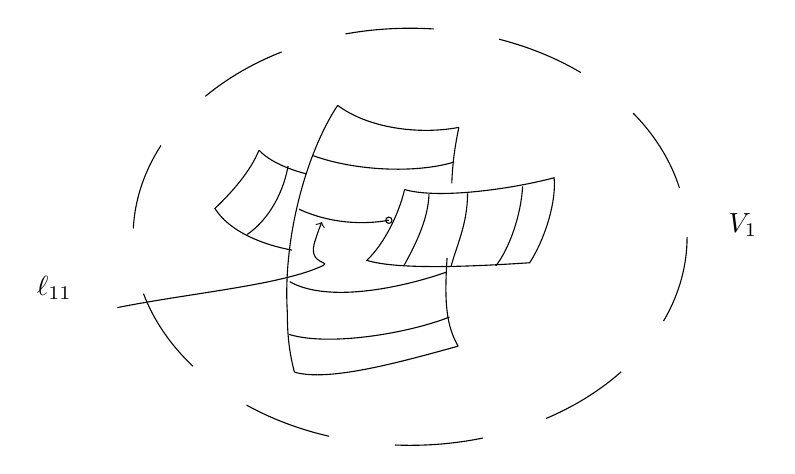
\begin{tikzpicture}[x=.01cm,y=-.01cm]
\draw[dash pattern=on 32pt off 24pt] (352,265) ellipse (352 and 265);
\draw (160,155)..controls (149,182) and (126,208)..(104,229)..controls (122,258) and (164,275)..(202,282);
\draw (160,155)..controls (174,170) and (200,180)..(220,185);
\draw (197,175)..controls (189,218) and (166,248)..(145,262);
\draw (260,98)..controls (222,155) and (190,263)..(196,361)..controls (196,388) and (198,410)..(205,437);
\draw (414,126)..controls (409,150) and (406,170)..(405,197);
\draw (399,292)..controls (395,353) and (399,379)..(413,404);
\draw (260,98)..controls (297,126) and (361,136)..(414,126);
\draw (205,437)..controls (249,450) and (344,423)..(413,404);
\draw (229,162)..controls (281,181) and (359,185)..(408,170);
\draw (211,230)..controls (250,248) and (292,250)..(325,244);
\draw (199,322)..controls (246,349) and (338,331)..(398,310);
\draw (198,389)..controls (250,405) and (352,387)..(402,367);
\draw (345,205)..controls (390,218) and (487,203)..(535,190)..controls (538,218) and (525,265)..(504,298)..controls (429,303) and (336,307)..(297,295)..controls (320,273) and (338,235)..(345,205);
\draw (376,211)..controls (375,242) and (360,273)..(344,302);
\draw (425,210)..controls (425,249) and (411,276)..(404,303);
\draw (495,201)..controls (493,238) and (478,280)..(461,302);
\draw (325,244) circle (4);
\draw[->] (-20,355)..controls (70,337) and (182,327)..(236,304)..controls (260,294) and (218,305)..(232,268)..controls (235,258) and (238,251)..(240,246);
\node at (-100,330) {$\ell_{11}$};\node at (775,250) {$V_1$};
\end{tikzpicture}}
\begin{center}\uline{Figure 7}\end{center}
\scanpage{34}
$V$ une sphère cohomologique
\[\Downarrow\]
\[\left\{\begin{gathered}
H^i(V_{\unsure{\eta|\gamma}})\longrightarrow H^{i-1}(V_s)\quad\text{un \uline{isom} si }\deleted{i,i+1\ne0,2n+1}\\
\inserted{\text{i.e. }i\ne0,2n\deleted{\unsure{+1}}}\\
\text{\uline{et }}\left\{\begin{array}{l}
H^0(V_{\unsure{\eta|\gamma}})\xleftarrow{\sim}\Lambda\\
H^{2n}(W_{\unsure{\eta|\gamma}})\longrightarrow H^{2n-1}(V_s)\quad\mathrm{inj}\text{ et conoyau }\deleted{\unsure{\ne}}\simeq\Lambda\\
\deleted{H^{2n+1}(V_s)\simeq\Lambda}
\end{array}\right.
\end{gathered}\right.\]
\margin{(\unsure{demand} $n\ge1$)}
\margin{$2n+1>n+1$}
\diagram{[\begin{tikzcd}[column sep=small,row sep=small]
\unsure{0}\arrow[r]&H^{2n}W_{\unsure{\eta|\gamma}})\arrow[r,no head]\arrow[d,equals]&H^{2n-1}(V_s)\arrow[r,no head]&H^{2n+1}(V)\arrow[r,no head]&H^{2n+1}(V_{\unsure{\eta|\gamma}})\arrow[r,no head]\arrow[d,equals]&H^{2n}(V_s)\arrow[r,no head]\arrow[d,equals]&0\\
&0&&&0&0\\
&\text{si }n\ge2&&&\text{si }n>1
\end{tikzcd}]}
\diagram{\begin{tikzcd}[row sep=large]
\text{si on suppose de plus que l'on a ``singularité isolée''}\arrow[d,Rightarrow,very thick]\\
H^i(V_s)=0\quad\text{si }i\ne0,n-1,n
\end{tikzcd}}
\margin{$H^i(V_{\unsure{\xi|\bar s}})\xrightarrow{\sim}H^i(V_s)$}
\figure{\begin{tikzpicture}\draw (0,0)--(0,2.4);\end{tikzpicture}}
\margin{\unsure{-}}
\mspage{33}
\scanpage{35}
\uline{Inconvénient sérieux} de la \unsure{solution|notation}
$\unsure{\operatorname{ad}^{n}|\operatorname{ad}^{\circ}}(S,\unsure{J|I};\mathcal A)$ lorsque $\mathcal A$ satisfait $(\mathrm{AB}\,5)$, $\unsure{\mathfrak B|\mathfrak I}$ $S$ noethérien : les conditions de finitude naturelles (pour $\mathcal A$ loc \unsure{noeth}) sur des systèmes inductifs adiques, ou co. adiques, ou \unsure{fst ann. adiques}, ne semblent pas stables par \uline{conoyaux} [\unsure{dualemt}, dans $\unsure{\mathrm{cc}|\operatorname{ad}}(S,\unsure{J|I};\mathcal A)$ quand $\mathcal A$ satisfait $(\mathrm{AB}\,5^{\unsure{\alpha|*}})$, les \unsure{condns} de finitude artiniennes ne semblent pas stables par noyaux] !!

\deleted{\uline{Exemple} $A$ anneau [noeth], $f,g$ deux éléments de $A$, $M$ un objet de \deleted{\unsure{\(\mathcal A\)}} $\mathcal C$, \unsure{tel que} $(f,g)$ soit \unsure{$M$-régulier}. Soit
\[P=M_f/M=\varinjlim_n M/f^nM\]
($M/f^mM\longrightarrow M/f^nM$ est donné par $f^{n-m}$ ; le système inductif est à morphismes de transition injectifs). Soit
\[Q=\]
}
\mspage{34}
